% ================================================================
%  KANDA — M.Tech Minor Project Report
%  KANDA = Knowledge-driven Autonomous Navigation and Decision-making Agent
%  Full title: A Multimodal Embodied Robot Agent Powered by LLMs
%               with Hardware Aware Action Generation
%  RV College of Engineering, Bengaluru
%  Dept. of ISE — 2025-26
% ================================================================
\documentclass[12pt,a4paper,oneside]{report}

% ---------- PACKAGES ----------
\usepackage[utf8]{inputenc}
\usepackage[T1]{fontenc}
\usepackage{times}                        % Times New Roman
\usepackage{microtype}                    % fewer overfull boxes; smarter hyphenation/justification
\usepackage[left=1in,right=1in,top=1in,bottom=1in,headheight=15pt]{geometry}
\usepackage{setspace}                     % 1.5 line spacing
\usepackage{fancyhdr}                     % custom headers/footers
\usepackage{graphicx}
\graphicspath{{images/}}
\usepackage{amsmath,amssymb}
\usepackage{booktabs}                     % nice tables
\usepackage{longtable}                    % multi-page tables
\usepackage{array}
\usepackage{tabularx}
\usepackage{xltabular}     
\usepackage{float}  % multi-page tabularx
\usepackage{enumitem}                     % custom lists
\usepackage{xurl}                         % breakable URLs/paths (must load before hyperref)
\makeatletter
\g@addto@macro\UrlBreaks{\do\_}           % allow breaks at underscores inside \url/\path
\makeatother
\usepackage[hidelinks]{hyperref}
\usepackage{listings}                     % code blocks
\usepackage{xcolor}
\usepackage{caption}
\usepackage{titlesec}                     % chapter/section styling
\usepackage{tocloft}                      % ToC formatting
\usepackage[numbers]{natbib}              % numeric cites (matches \bibliographystyle{ieeetr})

% ---------- TOC TITLE FORMATTING ----------
\renewcommand{\cfttoctitlefont}{\hfill\fontsize{18}{22}\selectfont\bfseries}
\renewcommand{\cftaftertoctitle}{\hfill}
\setlength{\cftbeforetoctitleskip}{0pt}
\setlength{\cftaftertoctitleskip}{12pt}

\renewcommand{\cftloftitlefont}{\hfill\fontsize{18}{22}\selectfont\bfseries}
\renewcommand{\cftafterloftitle}{\hfill}
\setlength{\cftbeforeloftitleskip}{0pt}
\setlength{\cftafterloftitleskip}{12pt}

\renewcommand{\cftlottitlefont}{\hfill\fontsize{18}{22}\selectfont\bfseries}
\renewcommand{\cftafterlottitle}{\hfill}
\setlength{\cftbeforelottitleskip}{0pt}
\setlength{\cftafterlottitleskip}{12pt}
\usepackage{parskip}                      % paragraph spacing

% ---------- REPORT FORMATTING NOTE ----------
% Avoid long uninterrupted \texttt{...} runs (they do not line-break). Prefer nested
% itemize for identifier lists, \path|...| for long paths, or break lines manually.
\usepackage{tikz}                         % diagrams and flowcharts
\usetikzlibrary{shapes.geometric,arrows.meta,positioning,calc,fit,backgrounds}

% ---------- PAGE STYLE ----------
\onehalfspacing
\setlength{\parindent}{0pt}
\setlength{\parskip}{6pt}

% Project metadata
\newcommand{\ProjectTitle}{A Multimodal Embodied Robot Agent Powered by LLMs with Hardware Aware Action Generation}
\newcommand{\ShortTitle}{Multimodal Embodied Robot Agent}
\newcommand{\StudentName}{Sudarshan T S}
\newcommand{\USN}{1RV24SIT14}
\newcommand{\GuideName}{Prof. Sushmitha N}
\newcommand{\Dept}{Department of Information Science \& Engineering}
\newcommand{\College}{RV College of Engineering\textsuperscript{\textregistered}}
\newcommand{\AcademicYear}{2025--26}

% ---------- HEADER / FOOTER ----------
% Default page style set to fancy (activated for main chapters)
\pagestyle{fancy}
\fancyhf{}
\renewcommand{\headrulewidth}{3pt}
\renewcommand{\footrulewidth}{3pt}
% Redefine chaptermark to only store chapter title (no "Chapter N.")
\renewcommand{\chaptermark}[1]{\markboth{#1}{}}
% Suppress sectionmark so it doesn't override the header
\renewcommand{\sectionmark}[1]{}
% Left header: chapter name only  |  Right header: short project title
\fancyhead[L]{\small\leftmark}
\fancyhead[R]{\small\ShortTitle}
\fancyfoot[L]{\small M.Tech in Information Technology}
\fancyfoot[C]{\small\AcademicYear}
\fancyfoot[R]{\small\thepage}

% Prelim style — no header/footer rules, just centered roman page number
\fancypagestyle{prelimstyle}{%
  \fancyhf{}
  \renewcommand{\headrulewidth}{0pt}
  \renewcommand{\footrulewidth}{0pt}
  \fancyfoot[C]{\small\thepage}
}

% ---------- CHAPTER / SECTION FORMATTING ----------
\titleformat{\chapter}[display]
  {\normalfont\bfseries}
  {\raggedright\fontsize{16}{19}\selectfont CHAPTER \thechapter}{0pt}
  {\centering\fontsize{18}{22}\selectfont}
\titlespacing*{\chapter}{0pt}{-20pt}{20pt}

\titleformat{\section}
  {\normalfont\large\bfseries}
  {\thesection}{1em}{}

\titleformat{\subsection}
  {\normalfont\normalsize\bfseries}
  {\thesubsection}{1em}{}

\titleformat{\subsubsection}
  {\normalfont\normalsize\bfseries\itshape}
  {\thesubsubsection}{1em}{}

% ---------- CODE LISTING STYLE ----------
\definecolor{codebg}{RGB}{245,245,245}
\definecolor{codegreen}{RGB}{0,128,0}
\definecolor{codegray}{RGB}{128,128,128}
\definecolor{codepurple}{RGB}{128,0,128}

\lstdefinestyle{pythonstyle}{
  backgroundcolor=\color{codebg},
  basicstyle=\ttfamily\footnotesize,
  breaklines=true,
  captionpos=b,
  commentstyle=\color{codegreen},
  keywordstyle=\color{codepurple}\bfseries,
  stringstyle=\color{red},
  numberstyle=\tiny\color{codegray},
  numbers=left,
  frame=single,
  framesep=3pt,
  xleftmargin=1em,
  showstringspaces=false,
}
\lstset{style=pythonstyle}

% ---------- VERBATIM BOX for architecture diagrams ----------
\usepackage{fancyvrb}

% ================================================================
\begin{document}

% ---- Front Matter (roman numerals, first 5 pages empty) ----
\pagenumbering{roman}
\pagestyle{empty}
% ================================================================
    %  00_prelims.tex — Title, Certificate, Acknowledgement, Abstract,
    %                    ToC, List of Figures/Tables, Glossary
    % ================================================================

    % ---- TITLE PAGE ----
    \begin{titlepage}
        \begin{center}
        \vspace*{1cm}
    
        {\large\bfseries Minor Project Report}\\[4pt]
        {\large\bfseries on}\\[8pt]
        {\Large\bfseries ``\ProjectTitle''}\\[20pt]
    
        {\large\bfseries MIT422P}\\[24pt]
    
        Submitted by\\[6pt]
        {\large\bfseries \StudentName}\\
        \USN\\[24pt]
    
        Under the Guidance of\\[6pt]
        {\large\bfseries \GuideName}\\
        Assistant Professor\\
        \Dept\\
        \College\\
        Bengaluru-560059\\[24pt]
    
        Submitted in partial fulfillment for the award of degree of\\[6pt]
        {\large\bfseries MASTER OF TECHNOLOGY}\\
        in\\
        {\large\bfseries INFORMATION TECHNOLOGY}\\[12pt]
    
        \MakeUppercase{\Dept}\\
        \MakeUppercase{\College}\\[6pt]
        \AcademicYear
    
        \end{center}
        \end{titlepage}
    
        % ---- CERTIFICATE (placeholder) ----
        \newpage
        \thispagestyle{empty}
        \begin{center}
        {\Large\bfseries\College}\\[4pt]
        {\small(Autonomous Institution Affiliated to Visvesvaraya Technological University, Belagavi)}\\[12pt]
        {\large\bfseries\MakeUppercase{\Dept}}\\
        Bengaluru--560059\\[20pt]
        {\Large\bfseries CERTIFICATE}
        \end{center}
        \vspace{12pt}
        Certified that the minor project work titled ``\ProjectTitle'' carried out by \textbf{\StudentName}, \USN, a bonafide student, submitted in partial fulfillment for the award of Master of Technology in Information Technology of Visvesvaraya Technological University, Belagavi, during the academic year \AcademicYear. It is certified that all corrections/suggestions indicated during the viva have been incorporated in the report. The project report has been approved as it satisfies the academic requirements in respect of the project work prescribed for the said degree.
    
        \vspace{36pt}
        \begin{tabular}{p{0.45\textwidth}p{0.45\textwidth}}
        \textbf{\GuideName} & \textbf{Dr. G.\,S.\,Mamatha} \\
        Internal Guide & Head of Department \\
        Assistant Professor & \Dept \\
        \Dept & \\
        \end{tabular}
    
        \vspace{36pt}
        \noindent\textbf{External Examiner:}\hfill Date: \rule{3cm}{0.4pt}
    
        % ---- DECLARATION ----
        \newpage
        \thispagestyle{empty}
        \begin{center}
        {\Large\bfseries\College}\\[4pt]
        {\small(Autonomous Institution Affiliated to Visvesvaraya Technological University, Belagavi)}\\[12pt]
        {\large\bfseries\MakeUppercase{\Dept}}\\
        Bengaluru--560059\\[20pt]
        {\Large\bfseries DECLARATION}
        \end{center}
        \vspace{12pt}
        I, \StudentName, student of M.Tech in Information Technology, Department of ISE, \College, Bengaluru declare that the Minor Project titled ``\ProjectTitle'', has been carried out by me and submitted in partial fulfillment of the requirements for the award of the degree of Master of Technology in Information Technology.
    
        I further declare that the project work is a result of my own effort and has not been submitted to any other university or institution for the award of any degree or diploma.
    
        \vspace{36pt}
        \begin{flushright}
        \textbf{\StudentName}\\
        Information Technology\\
        \Dept\\
        \College, Bengaluru-59
        \end{flushright}
    
        % ---- ACKNOWLEDGEMENT ----
        \newpage
        \thispagestyle{empty}
        \begin{center}
        {\Large\bfseries ACKNOWLEDGEMENT}
        \end{center}
        \addcontentsline{toc}{chapter}{Acknowledgement}
        \vspace{12pt}
    
        It needs more than these few words to express the immense gratitude and profound thanks to the people who gave all their valuable comments, suggestions and encouragement, making this work cruise smoothly along the path and rewarding the effort with success.
    
        I would like to express sincere gratitude to my guide, \textbf{\GuideName}, Assistant Professor, \Dept, \College, Bengaluru, for valuable guidance, expert review and constant encouragement in choosing this domain and support throughout the project.
    
        I would also like to express my sincere gratitude to \textbf{Dr.\ Padmashree~T}, Associate Professor and Associate Dean (PG Studies) and \textbf{Dr.\ G.\,S.\,Mamatha}, Professor and Head of the Department, Information Science \& Engineering, \College, Bengaluru, for the encouragement and support for the project.
    
        I thank \textbf{Dr.\ K\,N\,Subramanya}, Principal, \College, Bengaluru, for his valuable input for the project and for his moral support.
    
        I also thank my family and all the faculty members of the \Dept\ for their constant support and encouragement. Lastly, I would like to thank my professors, staff of ISE Department and colleagues who gave their valuable suggestions in the improvement of my project.
    
        \begin{flushright}
        \textbf{\StudentName}\\
        Information Technology\\
        Dept.\ of ISE\\
        \College, Bengaluru-59
        \end{flushright}
    
        % ---- ABSTRACT ----
        \newpage
        \thispagestyle{empty}
        \begin{center}
        {\Large\bfseries ABSTRACT}
        \end{center}
        \addcontentsline{toc}{chapter}{Abstract}
        \vspace{12pt}
    Autonomous mobile robots have traditionally relied on rule-based control systems that map sensor inputs to motor outputs through hand-crafted conditional logic. While effective for narrow, well-defined environments, such systems lack the ability to reason about novel situations, interpret ambiguous stimuli, or adapt behaviour based on contextual understanding. Simultaneously, Large Language Models (LLMs) have demonstrated remarkable contextual reasoning and structured output generation capabilities, but deploying them for real-time robot control requires bridging the semantic gap between language-based reasoning and physical hardware constraints. Without explicit hardware grounding, LLMs may generate physically impossible, unsafe, or malformed commands that cannot be executed by the robot's actuators.

    In this work, I present Knowledge-driven Autonomous Navigation and Decision-making Agent (KANDA), a multimodal embodied robot agent powered by LLMs with hardware-aware action generation. The system implements a dual-processor architecture in which an ESP32 microcontroller serves as the physical executor (body) handling real-time sensor acquisition and motor control, while a Raspberry Pi serves as the cognitive reasoner (brain) running Groq Llama~3.3 for text reasoning and NVIDIA NIM Llama~3.2 Vision for visual understanding. The system operates as a closed-loop sense--reason--validate--act pipeline: three ultrasonic sensors measure the environment, telemetry is transmitted via UART to the Raspberry Pi, a hardware-description prompt encoding the robot's capabilities and constraints aligns model behaviour with the physical platform, the model returns a structured JSON motion command, and a deterministic safety layer validates and clamps that command before driving the motors, closing the gap between open-ended language-model outputs and hard actuator constraints. The safety validator enforces an action whitelist, clamps speed to the permissible range, and substitutes a safe fallback on any validation failure. The ESP32 firmware implements dual-mode operation, automatically falling back to rule-based obstacle avoidance when the LLM is unavailable. The system was built on commodity hardware at a total cost below \$77, demonstrating that LLM-driven embodied intelligence is achievable without specialised robotic platforms or GPU-equipped onboard computers.
    
    
        % ---- TABLE OF CONTENTS ----
        \newpage
        \pagestyle{fancy}
        \fancypagestyle{plain}{%
        \fancyhf{}
        \renewcommand{\headrulewidth}{3pt}
        \renewcommand{\footrulewidth}{3pt}
        \fancyhead[C]{\hspace{0pt}}%
        \fancyfoot[L]{\small M.Tech in Information Technology}
        \fancyfoot[C]{\small\AcademicYear}
        \fancyfoot[R]{\small\thepage}
        }
        \tableofcontents
    
     % ---- LIST OF FIGURES ----
    \clearpage
    \phantomsection
    \addcontentsline{toc}{chapter}{List of Figures}
    \listoffigures

    % ---- LIST OF TABLES ----
    \clearpage
    \phantomsection
    \addcontentsline{toc}{chapter}{List of Tables}
    \listoftables
    
        % ---- GLOSSARY ----
        \newpage
        \begin{center}
        {\Large\bfseries GLOSSARY}
        \end{center}
        \addcontentsline{toc}{chapter}{Glossary}
        \vspace{12pt}
    
    \begin{longtable}{@{}l@{\hspace{1em}:\hspace{1em}}l@{}}
    \textbf{Term} & \textbf{Description} \\[4pt]
    KANDA  & Knowledge-driven Autonomous Navigation and Decision-making Agent \\
        LLM    & Large Language Model \\
        AI     & Artificial Intelligence \\
        API    & Application Programming Interface \\
        JSON   & JavaScript Object Notation \\
        UART   & Universal Asynchronous Receiver-Transmitter \\
        GPIO   & General Purpose Input/Output \\
        PWM    & Pulse Width Modulation \\
        I2C    & Inter-Integrated Circuit \\
        OLED   & Organic Light-Emitting Diode \\
        BMS    & Battery Management System \\
        DFD    & Data Flow Diagram \\
        SRS    & Software Requirement Specification \\
        ESP32  & Espressif Systems 32-bit Microcontroller \\
        HC-SR04 & Ultrasonic Distance Sensor Module \\
        TB6612FNG & Toshiba Dual H-Bridge Motor Driver IC \\
        SSD1306 & Solomon Systech OLED Display Driver \\
        LiPo   & Lithium Polymer (battery) \\
        LEDC   & LED Control (ESP32 PWM peripheral) \\
        NLP    & Natural Language Processing \\
        IoT    & Internet of Things \\
        SLAM   & Simultaneous Localisation and Mapping \\
        USB    & Universal Serial Bus \\
        CSV    & Comma-Separated Values \\
        \end{longtable}

\listoffigures
\listoftables
\clearpage

% ---- Main Chapters (arabic numerals, full header/footer) ----
\pagenumbering{arabic}
\pagestyle{fancy}
% Redefine 'plain' for chapter opening pages with thick rules
\fancypagestyle{plain}{%
  \fancyhf{}
  \renewcommand{\headrulewidth}{3pt}
  \renewcommand{\footrulewidth}{3pt}
  \fancyhead[C]{\hspace{0pt}}% force header rule
  \fancyfoot[L]{\small M.Tech in Information Technology}
  \fancyfoot[C]{\small\AcademicYear}
  \fancyfoot[R]{\small\thepage}
}
% ================================================================
%  Chapter 1 — Introduction
%  KANDA (Knowledge-driven Autonomous Navigation and Decision-making Agent):
%  A Multimodal Embodied Robot Agent Powered by LLMs with Hardware Aware Action Generation
% ================================================================
\chapter{Introduction}
\label{ch:intro}

This chapter introduces \textbf{Knowledge-driven Autonomous Navigation and Decision-making Agent (KANDA)}, a multimodal embodied robot agent powered by Large Language Models (LLMs) with hardware-aware action generation. The chapter discusses the context of embodied artificial intelligence, its global relevance, the specific technical problem addressed, and the objectives, scope and methodology of the project. The organisation of the report is presented at the end of the chapter.

%-------------------------------------------------------------------
\section{Overview of KANDA}
\label{sec:overview}

The field of robotics has historically relied on rule-based control systems that map sensor inputs to motor outputs through hand-crafted conditional logic. While effective for narrow, well-defined environments, such systems lack the ability to reason about novel situations, interpret ambiguous stimuli, or adapt their behaviour based on contextual understanding. A mobile robot encountering an unexpected obstacle configuration must either have a pre-programmed response for that exact scenario or fail ungracefully.

Recent advances in Large Language Models (LLMs) have demonstrated remarkable capabilities in natural language understanding, contextual reasoning, and structured output generation~\cite{vaswani2017attention}. These capabilities suggest a paradigm shift in robot control: rather than encoding every possible scenario in conditional logic, a robot can describe its sensory state to an LLM and receive a contextually appropriate action command in return. This approach, termed \textit{embodied AI}, bridges the gap between language-based reasoning and physical action execution~\cite{driess2023palme}.

KANDA addresses this opportunity by implementing a complete embodied robot agent in which an ESP32 microcontroller serves as the physical executor (body) and a Raspberry Pi running a Gemini LLM serves as the cognitive reasoner (brain). The system operates as a closed-loop sense--reason--validate--act pipeline: ultrasonic sensors measure the environment, sensor telemetry is transmitted to the Raspberry Pi via UART, a hardware-aware prompt is constructed and sent to the Gemini LLM, the returned JSON command is validated through a safety layer, and the validated command drives the motors. If the LLM fails or times out, the system gracefully degrades to rule-based obstacle avoidance, ensuring continuous safe operation.

%-------------------------------------------------------------------
\subsection{Embodied Intelligence Architecture}
\label{subsec:architecture}

KANDA operates as a three-layer processing architecture:

\textbf{Layer 1, Sensing \& Communication:}
Three HC-SR04 ultrasonic sensors (front, left, right) measure distances to obstacles at each control cycle. The ESP32 reads sensor values, formats front/left/right ranges and the current action label into a single telemetry line, and transmits this data over UART at 115,200 baud to the Raspberry Pi. Voltage dividers on each ECHO pin convert the 5V HC-SR04 output to approximately 2.5V, protecting the 3.3V-tolerant ESP32 GPIO pins.

\textbf{Layer 2, Reasoning \& Decision:}
The Raspberry Pi receives the telemetry and constructs a hardware-description prompt that communicates the robot's physical capabilities, current sensor readings, valid action vocabulary, speed constraints, and safety rules to the Gemini LLM. The model generates a single JSON object specifying the next action and speed. A safety validator then checks the command against a whitelist of valid actions and clamps speed to the permissible range $[0, 255]$. Any invalid command is replaced with a safe stop.

\textbf{Layer 3, Execution \& Feedback:}
The validated JSON command is transmitted back to the ESP32 over serial. The ESP32 parses the command and drives the TB6612FNG dual motor driver accordingly, while simultaneously displaying the current state on an SSD1306 OLED screen. The firmware implements dual-mode operation: AI\_MODE when valid commands arrive from the Pi, and AUTO\_MODE (rule-based obstacle avoidance) when the Pi is silent for longer than a configured timeout.

%-------------------------------------------------------------------
\subsection{Global Scenario}
\label{subsec:global}

The global robotics market is undergoing a transformation driven by the convergence of advances in foundation models, affordable embedded hardware, and edge computing. The International Federation of Robotics reported that over 500,000 new industrial robots were installed worldwide in 2023, while the service robotics sector grew by 48\% in unit sales~\cite{ifr2024report}. Simultaneously, the emergence of multimodal LLMs such as GPT-4, Gemini, and Claude has enabled language-conditioned robot control, where natural language serves as the interface between human intent and physical action~\cite{brohan2023rt2}.

Research efforts including SayCan~\cite{ahn2022saycan}, PaLM-E~\cite{driess2023palme}, and RT-2~\cite{brohan2023rt2} have demonstrated that LLMs can ground their language understanding in physical affordances, generating robot actions that respect hardware constraints. However, these systems typically require expensive robotic platforms, cloud-scale compute, or proprietary hardware. KANDA occupies the gap between research prototypes and educational platforms by implementing LLM-driven embodied intelligence on commodity hardware (ESP32 + Raspberry Pi) at a total cost below \$50, making embodied AI accessible for education, research, and rapid prototyping.

%-------------------------------------------------------------------
\subsection{Societal Relevance}
\label{subsec:societal}

Embodied AI agents with natural language understanding have direct societal applications:

\begin{itemize}[nosep]
  \item \textbf{Assistive robotics:} Indoor companion robots that can understand spoken instructions and navigate home environments safely benefit elderly and mobility-impaired individuals.
  \item \textbf{Education:} A low-cost platform that demonstrates LLM-robot integration provides hands-on learning for robotics, embedded systems, and AI courses.
  \item \textbf{Search and rescue:} Robots that can reason about sensor data and adapt to novel obstacle configurations are valuable in disaster response scenarios.
  \item \textbf{Safety research:} The safety validation layer demonstrates how to constrain AI-generated actions before physical execution, contributing to the broader discourse on safe AI deployment.
\end{itemize}

From an engineering perspective, the project integrates embedded systems programming (ESP32/Arduino), hardware interfacing (ultrasonic sensors, motor drivers, voltage dividers), inter-processor communication (UART/serial), cloud API integration (Gemini), and software safety engineering into a single cohesive system, making it a comprehensive study in applied software and hardware co-design.

%-------------------------------------------------------------------
\subsection{Problem Area}
\label{subsec:problem_area}

Current approaches to autonomous mobile robot navigation suffer from three interrelated limitations:

\begin{enumerate}[label=\arabic*.]
  \item \textbf{Rigidity of rule-based control:} Traditional obstacle avoidance algorithms use fixed distance thresholds and pre-programmed turning sequences. When the environment presents a configuration not anticipated by the programmer (e.g., a narrow corridor with asymmetric obstacles), the robot either oscillates between conflicting rules or fails to find a viable path. The system cannot \textit{reason} about the spatial arrangement or consider alternative strategies.

  \item \textbf{Disconnect between language models and physical hardware:} General-purpose LLMs possess strong reasoning capabilities but have no inherent knowledge of a specific robot's physical constraints. Asking a language model ``What should the robot do?'' without communicating the robot's sensor state, actuator capabilities, and safety limits produces hallucinated or physically impossible commands~\cite{ahn2022saycan}. Bridging this semantic gap requires a carefully engineered prompt that grounds the model in hardware reality.

  \item \textbf{Absence of safety guarantees:} LLM outputs are probabilistic and can occasionally produce malformed, out-of-vocabulary, or unsafe commands. A system that directly executes raw LLM output on physical hardware risks motor stalls, collisions, overcurrent conditions, or damage to the robot and its environment. A systematic validation layer between the LLM and the actuators is essential but is absent in most prototype systems.
\end{enumerate}

KANDA addresses all three problems through its hardware-aware prompting, structured JSON command interface, and mandatory safety validation layer.

%-------------------------------------------------------------------
\section{Specific Details of KANDA}
\label{sec:specific}

KANDA is implemented as a dual-processor system with the following key technical characteristics:

\textbf{Hardware platform:}
\begin{itemize}[nosep]
  \item ESP32 DevKit microcontroller (dual-core Tensilica Xtensa, 240\,MHz, Wi-Fi/Bluetooth)
  \item TB6612FNG dual H-bridge motor driver with PWM speed control (1\,kHz, 8-bit resolution)
  \item 3$\times$ HC-SR04 ultrasonic distance sensors with 1\,k$\Omega$ + 1\,k$\Omega$ voltage dividers
  \item SSD1306 OLED display (128$\times$64, I2C at address \texttt{0x3C})
  \item 7.4V LiPo battery with BMS and buck converter (5V regulated output to ESP32)
  \item Raspberry Pi (Python runtime, Gemini API client, safety validator)
\end{itemize}

\textbf{Communication:}
\begin{itemize}[nosep]
  \item UART serial at 115,200 baud between ESP32 and Raspberry Pi
  \item ESP32 transmits telemetry lines matching \path|F:<cm> L:<cm> R:<cm> -> <ACTION>|
  \item Raspberry Pi transmits commands as one JSON object per line, schema \path|{"action":"<cmd>","speed":<int>}|
  \item Auto-mode detection: if no valid JSON received within timeout, ESP32 reverts to standalone operation
\end{itemize}

\textbf{AI reasoning:}
\begin{itemize}[nosep]
  \item Google \textbf{Gemini 2.5 Flash} (\texttt{gemini-2.5-flash}): strong reasoning and latency characteristics suited to closed-loop robotics; configurable via \texttt{GEMINI\_MODEL}
  \item \textbf{Alignment:} hardware-description prompt aligns model outputs with actuator affordances; low temperature and JSON-only response format constrain decoding; the validator provides runtime alignment by mapping every candidate command to a safe, whitelisted action and bounded speed~\cite{huang2023grounded,ahn2022saycan}
  \item Hardware-description prompt with explicit action vocabulary, speed range, and safety rules
  \item Temperature 0.2 for deterministic JSON output
  \item Maximum 64 output tokens (command is a single JSON object)
  \item 2-second control loop interval
\end{itemize}

\textbf{Safety validation:}
\begin{itemize}[nosep]
  \item Action whitelist (fixed vocabulary):
  \begin{itemize}[nosep,leftmargin=1.25em]
    \item \texttt{forward}, \texttt{backward}, \texttt{left}, \texttt{right}
    \item \texttt{slight\_left}, \texttt{slight\_right}, \texttt{stop}
  \end{itemize}
  \item Speed clamping to $[0, 255]$
  \item Type checking on all command fields
  \item Fallback on any validation failure to \path|{"action":"stop","speed":0}|
\end{itemize}

\textbf{Firmware modes:}
\begin{itemize}[nosep]
  \item \texttt{AI\_MODE}: Raspberry Pi sends JSON commands; ESP32 executes them
  \item \texttt{AUTO\_MODE}: Standalone rule-based obstacle avoidance (Phase~2 behaviour)
  \item Automatic switching: valid JSON reception $\rightarrow$ AI\_MODE; timeout $\rightarrow$ AUTO\_MODE
\end{itemize}

%-------------------------------------------------------------------
\section{Literature Review}
\label{sec:litreview}

\textbf{\cite{driess2023palme} Driess, D., et al.\ (2023). PaLM-E: An Embodied Multimodal Language Model.}
Presented PaLM-E, a 562-billion parameter multimodal language model that integrates real-world sensor modalities (images, state estimation, scene representations) directly into the language model, enabling embodied reasoning for robot manipulation and navigation. PaLM-E demonstrated that a single large model can ground language in physical observations without task-specific fine-tuning. KANDA shares the principle of grounding language models in sensor observations but achieves this through structured prompting rather than end-to-end multimodal training, enabling deployment on commodity hardware.

\textbf{\cite{ahn2022saycan} Ahn, M., et al.\ (2022). Do As I Can, Not As I Say: Grounding Language in Robotic Affordances.}
Introduced SayCan, which combines an LLM's language understanding with a learned affordance model to select actions that are both useful (according to the LLM) and feasible (according to the robot's current state). SayCan demonstrated a 74\% improvement in plan execution success rate on a mobile manipulator. KANDA adopts SayCan's principle of affordance grounding but implements it through explicit hardware-description prompts rather than learned value functions.

\textbf{\cite{brohan2023rt2} Brohan, A., et al.\ (2023). RT-2: Vision-Language-Action Models.}
Presented Robotic Transformer 2 (RT-2), which directly maps visual observations and language instructions to robot actions by fine-tuning a vision-language model on robot demonstration data. RT-2 achieved a 2$\times$ improvement in generalisation to unseen objects. KANDA's Phase~4 architecture targets similar vision-language-action capabilities but operates through API-based inference rather than on-device model execution.

\textbf{\cite{vemprala2024chatgpt} Vemprala, S., et al.\ (2024). ChatGPT for Robotics: Design Principles and Model Abilities.}
Evaluated ChatGPT's ability to generate robot control code and task plans when provided with API documentation and environmental context. The study established design principles for effective robot-LLM interaction, including the importance of well-structured prompts and iterative dialogue. KANDA's context builder module implements these prompt engineering principles in the robotics domain.

\textbf{\cite{liang2023code} Liang, J., et al.\ (2023). Code as Policies: Language Model Programs for Embodied Control.}
Proposed using LLMs to generate executable robot control code rather than high-level plans. The approach enables compositional and expressive robot behaviours beyond fixed action primitives. KANDA currently uses a fixed action vocabulary with JSON commands but the architecture supports extension to code-as-policy in future phases.

\textbf{\cite{singh2023progprompt} Singh, I., et al.\ (2023). ProgPrompt: Program Generation for Situated Robot Task Planning.}
Presented ProgPrompt, which generates situated robot task plans as executable programs by providing the LLM with environment-specific function signatures and state descriptions. KANDA's hardware-description prompt follows a similar structure: explicit function documentation (valid actions), state description (sensor readings), and constraints (safety rules).

\textbf{\cite{huang2023grounded} Huang, W., et al.\ (2023). Grounded Decoding: Guiding Text Generation with Grounded Models.}
Proposed grounded decoding, which combines a language model's token probabilities with a grounding model's feasibility scores at each decoding step. KANDA's safety validator operates on a similar principle but at the command level rather than the token level: the LLM generates a complete command, and the validator checks its feasibility before execution.

\textbf{\cite{wu2023tidybot} Wu, J., et al.\ (2023). TidyBot: Personalised Robot Assistance with LLMs.}
Demonstrated a household robot that uses LLMs to infer user preferences for object placement from a small number of examples. TidyBot showed that LLMs can generalise from limited demonstrations to novel situations in physical environments. KANDA's architecture supports similar personalisation through the user speech input slot in the context builder.

\textbf{\cite{hu2023llmplanner} Hu, Y., et al.\ (2023). LLM-Planner: Few-Shot Grounded Planning for Embodied Agents.}
Proposed LLM-Planner for generating grounded action plans from natural language instructions with few-shot examples. The system uses environmental feedback to dynamically re-plan when actions fail. KANDA's control loop similarly incorporates environmental feedback (sensor telemetry) at each reasoning cycle, enabling continuous re-planning.

\textbf{\cite{wake2023gptrobot} Wake, N., et al.\ (2023). ChatGPT Empowered Long-Step Robot Control.}
Demonstrated multi-step robot task execution by decomposing complex instructions into sequential action primitives using ChatGPT. KANDA shares the decomposition approach but operates at a single-step granularity (one action per reasoning cycle) to maintain real-time responsiveness.

\textbf{\cite{zeng2023socratic} Zeng, A., et al.\ (2023). Socratic Models: Composing Zero-Shot Multimodal Reasoning.}
Proposed Socratic Models, where multiple foundation models (language, vision, audio) communicate through natural language to solve multimodal tasks without task-specific training. KANDA's Phase~4 architecture envisions a similar composition: a vision model processes camera frames, a speech model transcribes user commands, and the LLM integrates all modalities for action generation.

\textbf{\cite{espressif2023esp32} Espressif Systems (2023). ESP32 Technical Reference Manual.}
The official hardware reference for the ESP32 microcontroller, documenting GPIO capabilities, strapping pin constraints, LEDC PWM peripheral, UART controllers, and I2C interface. KANDA's pin configuration and firmware design directly follow the constraints documented in this manual.

%-------------------------------------------------------------------
\section{Problem Statement}
\label{sec:problem}

Traditional mobile robot systems implement navigation through hard-coded conditional logic: if the front sensor reads below a threshold, turn; if a side sensor detects proximity, steer away. While functional in simple environments, this approach is fundamentally limited in three ways. First, the rule set cannot be exhaustive: any spatial configuration not explicitly anticipated produces either an incorrect response or a deadlock, and the number of possible obstacle configurations in real-world environments is effectively infinite. Second, the system cannot leverage contextual understanding: a robot approaching a narrow doorway should slow down and align carefully, while the same frontal distance reading in an open room warrants a simple course correction, yet threshold-based systems treat both situations identically. Third, the system offers no natural language interface: a user cannot simply say ``go to the kitchen'' or ``avoid that area'' because the system has no mechanism to interpret semantic intent and translate it into a sequence of physical actions.

Simultaneously, Large Language Models have demonstrated strong contextual reasoning and structured output generation capabilities, but deploying them for real-time robot control introduces its own set of challenges. An LLM has no inherent knowledge of a particular robot's physical dimensions, sensor coverage angles, motor response characteristics, or safety limits. Without explicit hardware grounding, the model may generate physically impossible commands (e.g., ``fly upward''), unsafe actions (e.g., ``full speed forward'' when an obstacle is 10\,cm away), or malformed outputs that cannot be parsed by the firmware. Furthermore, API-based LLM inference introduces variable latency (typically 1--5 seconds), requiring the system to maintain safe operation during reasoning intervals.

Hence, there is a need for an embodied robot system that combines LLM-based contextual reasoning with hardware-aware action generation, implements a mandatory safety validation layer between the model output and physical execution, provides graceful degradation to autonomous operation when the reasoning layer is unavailable, and operates on affordable commodity hardware suitable for educational and research applications.

%-------------------------------------------------------------------
\section{Objectives}
\label{sec:objectives}

The objectives of the KANDA project are as follows:

\begin{enumerate}[label=\arabic*.]
  \item \textbf{To design and implement a dual-processor robot architecture} in which an ESP32 microcontroller handles real-time sensor acquisition and motor control while a Raspberry Pi executes LLM-based cognitive reasoning, communicating via structured JSON over UART serial.

  \item \textbf{To develop a hardware-aware context builder} that constructs LLM prompts encoding the robot's physical capabilities, current sensor state, valid action vocabulary, speed constraints, and safety rules, enabling the language model to generate physically grounded commands.

  \item \textbf{To implement a safety validation layer} that verifies every LLM-generated command against a whitelist of valid actions, clamps speed to the permissible hardware range, and substitutes a safe fallback command upon any validation failure, ensuring that no unchecked AI output reaches the physical actuators.

  \item \textbf{To build a dual-mode firmware} for the ESP32 that operates in AI\_MODE when receiving valid commands from the Raspberry Pi and automatically falls back to rule-based AUTO\_MODE upon communication timeout, guaranteeing continuous safe operation independent of LLM availability.

  \item \textbf{To demonstrate the complete sense--reason--validate--act loop} on a physical robot platform using commodity hardware (total cost below \$50), showing that LLM-driven embodied intelligence is achievable without specialised robotic platforms or GPU-equipped onboard computers.

  \item \textbf{To evaluate the system} through test scenarios including open corridor navigation, obstacle avoidance, narrow passage traversal, and LLM failure recovery, demonstrating that hardware-aware prompting produces contextually appropriate actions while the safety layer prevents unsafe execution.
\end{enumerate}

%-------------------------------------------------------------------
\section{Scope}
\label{sec:scope}

\textbf{In scope:}
\begin{itemize}[nosep]
  \item Two-wheeled differential-drive robot platform with ultrasonic obstacle detection
  \item Dual-processor architecture (ESP32 executor + Raspberry Pi reasoner)
  \item LLM integration via Google Gemini API with hardware-aware prompting
  \item Safety validation layer with action whitelisting and speed clamping
  \item Dual-mode firmware with automatic AI/autonomous switching
  \item UART serial communication protocol between processors
  \item Real-time OLED status display
  \item Indoor navigation scenarios on flat surfaces
\end{itemize}

\textbf{Out of scope:}
\begin{itemize}[nosep]
  \item Outdoor navigation or uneven terrain traversal
  \item Vision-based perception (camera integration is Phase~4 future work)
  \item Speech recognition and synthesis (Phase~4 future work)
  \item Multi-robot coordination or swarm behaviour
  \item On-device LLM inference (all reasoning uses cloud API)
  \item Simultaneous localisation and mapping (SLAM)
  \item Manipulation tasks (no robotic arm)
\end{itemize}

%-------------------------------------------------------------------
\section{Methodology}
\label{sec:methodology}

The project follows a phased iterative development methodology:

\textbf{Phase~1, Conceptual Design \& Literature Review:} Study of embodied AI architectures, LLM-robot integration frameworks (SayCan, PaLM-E, RT-2), ESP32 hardware constraints, motor driver interfacing, and ultrasonic sensor characteristics. Identification of the hardware-grounding gap as the primary technical challenge.

\textbf{Phase~2, Embodiment Layer (Hardware + Rule-Based Control):} Assembly of the physical robot platform including ESP32, TB6612FNG motor driver, three HC-SR04 ultrasonic sensors with voltage dividers, SSD1306 OLED, and LiPo power system. Implementation of standalone rule-based obstacle avoidance firmware operating as a sense--decide--act--display loop. Validation of all hardware interfaces including PWM motor control, I2C display communication, and ultrasonic distance measurement accuracy.

\textbf{Phase~3, Intelligence Layer (LLM Integration):} Implementation of the Raspberry Pi AI layer including the UART bridge for serial communication with ESP32, the context builder for hardware-aware prompt construction, the Gemini LLM client with response parsing, and the safety validator. Integration of dual-mode firmware that accepts AI commands when available and falls back to autonomous operation otherwise. End-to-end testing of the complete sense--reason--validate--act pipeline.

\textbf{Phase~4, Multimodal Extension (Future Work):} Addition of camera input for visual perception, microphone for voice commands, and speaker for audio feedback. Extension of the context builder to include image and speech modalities. Implementation of task memory and multi-step planning.

%-------------------------------------------------------------------
\section{Organization of Report}
\label{sec:org}

The report is organized into the following chapters:

\textbf{Chapter~1, Introduction:} Background and motivation, global and societal relevance, problem statement, objectives, scope, methodology, and organisation of the report.

\textbf{Chapter~2, Theory and Concepts:} Theoretical foundations covering embodied AI, Large Language Models for robot control, sense--reason--act architectures, ultrasonic distance sensing, PWM motor control, UART serial communication, and safety validation in autonomous systems.

\textbf{Chapter~3, Software Requirement Specification:} Functional and non-functional requirements, product perspective and functions, user classes, system constraints, and hardware/software requirements.

\textbf{Chapter~4, High Level Design:} System architecture, design considerations, development methodology, data flow diagrams at levels~0, 1, and~2, and architectural strategies.

\textbf{Chapter~5, Detailed Design:} Module-level structure chart, detailed description of each module including ESP32 firmware, UART bridge, context builder, LLM client, safety validator, and orchestrator.

\textbf{Chapter~6, Implementation:} Languages and platforms, repository layout, UART/JSON protocol, firmware and Python implementation excerpts, integration difficulties, and build/run steps.

\textbf{Chapter~7, Software Testing:} Unit, integration, and system test procedures; traceability to functional requirements; limitations and future test automation.

\textbf{Chapter~8, Experimental Results and Conclusions:} Demonstration outcomes, timing parameters, discussion of limitations, and conclusions with Phase~4 future work.

\textbf{Chapter~9, Conclusion:} Objective-to-evidence mapping, engineering reflections, and closing remarks.

%-------------------------------------------------------------------
\section{Summary}
\label{sec:ch1summary}

This chapter presented the motivation, context, and design philosophy of KANDA, a multimodal embodied robot agent powered by LLMs with hardware-aware action generation. The key insight driving the project is that language models can serve as the reasoning brain of a physical robot provided they are explicitly grounded in the robot's hardware capabilities through structured prompts, and their outputs are validated through a safety layer before reaching the actuators. KANDA implements this insight as a dual-processor architecture where an ESP32 handles real-time sensing and motor execution while a Raspberry Pi running Gemini provides contextual reasoning at each control cycle. The problem statement articulates the limitations of rule-based control, the hardware-grounding gap in LLM-robot integration, and the absence of safety guarantees in existing prototype systems. The six project objectives span the dual-processor architecture, hardware-aware prompting, safety validation, dual-mode firmware, commodity hardware demonstration, and scenario-based evaluation. The chapter concluded with the scope boundaries, phased methodology, and the organization of the report through implementation, testing, results, and conclusion (Chapters~6--9).

% ================================================================
%  Chapter 2 — Theory and Concepts
%  KANDA (Knowledge-driven Autonomous Navigation and Decision-making Agent)
% ================================================================
\chapter{THEORY AND CONCEPTS}
\label{ch:theory}

Building a robot that listens, sees, thinks, and moves requires pulling ideas from several fields at once. This chapter lays out those ideas, not as a textbook survey, but tied directly to decisions I had to make while constructing KANDA. Why does the language model need to know the robot's sensor readings? Why can I not just send raw text to the motors? Why does the ESP32 need its own safety logic when the Pi is already running a validator? Each section answers one of these questions by grounding it in published work and then connecting it to my specific implementation choices.


%-------------------------------------------------------------------
\section{Embodied Artificial Intelligence}
\label{sec:embodied}

A language model sitting on a server can write poetry about walking, but it has never tripped over a cable. \textbf{Embodied AI} closes that gap; it insists that intelligent behaviour only makes sense when perception and action happen through a real body interacting with a physical world. The distinction matters practically: an embodied system must deal with noise from cheap sensors, latency over wireless links, and the fact that motors do not care about elegant sentences.


These systems cost tens or hundreds of thousands of dollars. KANDA asks a simpler question: can the \textit{behaviours} that matter for a desk-sized indoor robot (obstacle avoidance, voice commands, object search) run on a \$77 platform with no training data at all? The answer turns out to be yes, but only if I respect the old principle from Brooks~\cite{brooks1986robust} that fast reactive layers must sit beneath slow deliberative ones. My firmware reflex traces its lineage directly to subsumption architecture, even though the deliberation layer above it uses a 70-billion parameter model hosted in the cloud.


These systems cost tens or hundreds of thousands of dollars. KANDA asks a simpler question: can the \textit{behaviours} that matter for a desk-sized indoor robot (obstacle avoidance, voice commands, object search) run on a \$77 platform with no training data at all? The answer turns out to be yes, but only if we respect the old principle from Brooks~\cite{brooks1986robust} that fast reactive layers must sit beneath slow deliberative ones. Our firmware reflex traces its lineage directly to subsumption architecture, even though the deliberation layer above it uses a 70-billion parameter model hosted in the cloud.

%-------------------------------------------------------------------
\subsection{Affordance Grounding}
\label{subsec:affordance}

Gibson coined the term \textit{affordance} to describe what an environment offers a particular agent; a chair affords sitting for a human but not for a fish. In robotics, the question becomes: given a language command like ``put the cup on the shelf,'' which physical actions can this robot actually perform?

SayCan~\cite{ahn2022saycan} tackled this by training affordance functions from 68,000 demonstrations. When a user issued a command, the system combined the language model's preference with a learned feasibility score to pick actions the robot could physically execute. PaLM-E~\cite{driess2023palme} took a different route, embedding sensor tokens directly into the language model so it could reason about feasibility internally. RT-2~\cite{brohan2023rt2} pushed further; it fine-tuned a vision-language model end-to-end so that the model output was itself a motor command, eliminating the separate affordance filter.

I could not afford 68,000 demonstrations, a 562B model, or end-to-end fine-tuning. Instead, KANDA encodes affordances directly in the prompt: seven legal actions, a speed range of 0--255, and live ultrasonic distances. The model cannot propose ``fly'' or ``speed 500'' because the prompt tells it those do not exist. This is crude compared to learned affordances, but it costs nothing to maintain and catches most hallucinated actions before validation even runs.


%-------------------------------------------------------------------
\section{Large Language Models for Robot Control}
\label{sec:llm_robot}

Transformers~\cite{vaswani2017attention} revolutionised natural language processing by replacing recurrence with self-attention, enabling parallel training on massive corpora. The resulting models (GPT-4, Llama, Gemini) generate fluent text, but fluency does not imply physical feasibility. A model might confidently suggest ``accelerate to 400'' when the motor driver caps at 255.

The gap between linguistic competence and physical grounding defines the core challenge. Vemprala et al.~\cite{vemprala2024chatgpt} articulated this in 2024: successful LLM-robot integration requires (a)~a clear description of the robot's capabilities in the prompt, (b)~low-temperature sampling to suppress creative but dangerous outputs, and (c)~a post-generation filter that catches anything the prompt did not prevent. KANDA implements all three, though I arrived at this design through trial and error before reading their systematic treatment.


%-------------------------------------------------------------------
\subsection{Prompting as Interface Specification}
\label{subsec:prompting}

Rather than training models on robot data, several groups discovered that careful prompting alone can produce usable control outputs. Huang et al.~\cite{huang2022zeroshot} first demonstrated that language models serve as effective zero-shot planners when carefully framed. Liang et al.~\cite{liang2023code} framed the prompt as a Python API specification and let the model write policy code. Singh et al.~\cite{singh2023progprompt} went further, declaring robot functions and world state in the prompt so the model could generate situated programs.

Chain-of-thought prompting~\cite{wei2022cot} showed that forcing the model to ``think step by step'' improves multi-step planning. Yao et al.\ combined this with action execution in ReAct~\cite{yao2023react}, where the model alternates between reasoning traces and concrete actions, observing results before deciding the next step. Our visual search algorithm borrows this structure: capture a frame, describe it, decide whether the target is visible, then pick the next movement.

KANDA's prompt is deliberately simpler than these systems. I do not generate code or multi-step reasoning chains at inference time. The prompt specifies seven verbs, a numeric speed field, and current sensor readings. The model returns a single JSON line. This keeps the firmware parser trivial and the validator unambiguous.


%-------------------------------------------------------------------
\subsection{Grounded Decoding and Post-Hoc Validation}
\label{subsec:grounded}

Huang et al.~\cite{huang2023grounded} proposed an elegant idea: during token generation, multiply the language model's probability distribution by a grounding signal (e.g., a feasibility score from a physics model) so that infeasible tokens get suppressed before they even appear in the output. This requires access to the model's logits, something cloud APIs generally do not expose.

KANDA takes the conceptually similar but architecturally distinct approach of post-hoc validation. I let the model generate freely, then run a total function $V$ that either accepts the output (if action $\in$ whitelist and speed $\in [0,255]$) or replaces it with a stop command. The validator never raises an exception, never passes garbage downstream, and adds negligible latency ($<$1\,ms). It is less elegant than logit-level intervention, but works with any API, any model, and any future provider swap.


%-------------------------------------------------------------------
\section{Sense-Reason-Act Architecture}
\label{sec:sra}

Most autonomous robots follow a loop: read sensors, compute a decision, execute it, repeat. KANDA splits this across two processors running at wildly different speeds, and that split drives much of the architecture.

The ESP32 reads three ultrasonic sensors every 100\,ms, fast enough to catch a hand waving in front of the robot. The Raspberry Pi calls Groq or NVIDIA NIM over the network, which takes 1.5--4 seconds depending on server load and prompt length. If I forced the ESP32 to wait for every cloud response, the robot would lurch forward blindly during those seconds. Instead, the firmware runs its own obstacle-avoidance rules whenever the Pi has not sent a command recently (timeout: 3 seconds). The Pi's commands override these rules when they arrive, but the firmware never stops watching the sensors.


This is not a novel idea; Brooks described it in 1986~\cite{brooks1986robust}. What is new is layering a cloud-hosted 70B-parameter model on top of a \$4 microcontroller and still preserving sub-100\,ms reflexes. The trick is accepting that the LLM is advisory, not authoritative. It suggests; the validator approves; the firmware obeys, or overrides if the wall is too close.

%-------------------------------------------------------------------
\section{Proximate Sensing with Ultrasonic Rangefinders}
\label{sec:ultrasonic}

HC-SR04 modules are cheap, widely available, and good enough for indoor obstacle detection within 2--400\,cm. The Dynamic Window Approach~\cite{fox1997dwa} provides a formal basis for velocity-space obstacle avoidance; our threshold-based design simplifies this to a binary stop decision at 15\,cm. The principle is straightforward: a 40\,kHz burst leaves the transmitter, bounces off a surface, and returns to the receiver. The module holds an echo pin high for the round-trip duration $\Delta t$, and distance follows from $d = \frac{1}{2} \cdot 343 \cdot \Delta t$ metres at room temperature.

In practice, three issues dominated our debugging time. First, the 15-degree beam width means small objects at oblique angles go undetected. Second, running three sensors simultaneously causes cross-talk where one sensor picks up another's echo. We solved this by triggering them sequentially within each loop iteration. Third, the HC-SR04 outputs 5V echo pulses, but ESP32 GPIO pins tolerate only 3.3V. Resistor dividers on each echo line handle the level shift; without them, the ESP32 reads noise or risks input damage.

%-------------------------------------------------------------------
\section{PWM Actuation and Motor Drive}
\label{sec:pwm}

DC motors spin faster with higher average voltage. Rather than regulating actual voltage, we switch full supply on and off rapidly (Pulse Width Modulation) so that the motor sees an effective average proportional to the duty cycle. The ESP32's LEDC peripheral~\cite{espressif2023esp32} generates PWM signals with 8-bit resolution (0--255) at 1\,kHz, which is high enough that the motors hum rather than click.

The TB6612FNG dual H-bridge sits between the ESP32 logic and the motors. Two direction pins per channel set forward or reverse; one PWM pin per channel sets speed. For differential steering, equal duty on both channels drives straight; unequal duty turns gently; reversing one channel spins in place. KANDA maps abstract LLM verbs (\textit{forward}, \textit{slight\_left}, \textit{right}) to specific combinations of direction bits and PWM values in firmware, so the language model never deals with pin-level hardware.

%-------------------------------------------------------------------
\section{Inter-Processor Communication over UART}
\label{sec:uart}

UART serial at 115,200 baud connects the Raspberry Pi and ESP32 with just two wires (TX and RX, plus ground). No clock line, no protocol negotiation; bytes flow at the agreed rate with start and stop framing. I chose newline-terminated JSON as the message format for a practical reason: it is human-readable in a serial monitor, which saved hours during early integration when half the bugs were bad baud rates or swapped TX/RX wires.


The Pi sends one JSON object per line: \textit{\{"action":"forward","speed":120\}}. The ESP32 replies with sensor telemetry in a fixed ASCII format: \textit{F:30.5 L:21.0 R:16.4 -> FORWARD}. Both sides use newline as the message delimiter. ArduinoJson parses the inbound line on the ESP32; Python's \textit{json.loads} handles it on the Pi. The simplicity of this protocol (no handshake, no sequence numbers, no retransmission) means occasional dropped bytes produce a parse failure that the validator catches and maps to stop. Reliability through simplicity.

%-------------------------------------------------------------------
\section{Safety Validation for LLM-Generated Actions}
\label{sec:safety_theory}

Language models hallucinate. They invent actions that do not exist, propose speeds that exceed hardware limits, wrap JSON in markdown fences, or occasionally return poetry instead of motor commands. KANDA assumes every LLM output is adversarial until proven otherwise.

The validator implements four checks in sequence: (1)~is the output a dictionary with the right keys? (2)~is the action one of seven known verbs? (3)~can the speed field be parsed as an integer? (4)~is that integer within $[0,255]$? Failure at any stage produces a safe stop command. Speed values outside the range but otherwise valid get clamped rather than rejected, so ``speed 300'' becomes ``speed 255'' rather than a full stop. This design treats the validator as a total function: it always terminates, always returns a legal command, and never throws~\cite{huang2023grounded,ahn2022saycan}.

The firmware adds a second, independent safety layer. Even if the Pi's validator somehow passes a forward command while an obstacle sits 10\,cm ahead, the ESP32's own loop checks the front sensor and overrides with a stop. Two independent checks, running on separate processors, make single-point failure of safety essentially impossible for the collision case.

%-------------------------------------------------------------------
\section{Multimodal Extension}
\label{sec:multimodal}

Phase~4 of KANDA adds a camera, microphone, and speaker, turning it from a text-controlled rover into a multimodal agent. The conceptual basis draws from several 2022--2023 systems.

Wake et al.~\cite{wake2023gptrobot} showed that ChatGPT can plan multi-step robot actions in diverse environments when given adequate scene descriptions. Wu et al.~\cite{wu2023tidybot} built a robot that learns personal preferences via language, deciding where specific objects belong in a household. Zeng et al.~\cite{zeng2023socratic} composed separately trained models (vision, language, audio) by passing natural-language summaries between them, requiring no joint training. Huang et al.~\cite{huang2022innermonologue} fed observation text back into the planner so the robot could notice when actions failed and try alternatives.

KANDA's search algorithm combines these ideas: the vision model describes each captured frame, the text model decides whether the target is visible and which direction to explore next, and episodic memory prevents the robot from revisiting scenes it has already checked. The entire loop stays within the same validation boundary that governs simple motion commands, so even during a 20-step search, every individual movement passes through the safety validator before reaching the wheels.

%-------------------------------------------------------------------
\section{Summary}
\label{sec:ch2summary}

The theoretical basis of KANDA spans classical robotics and frontier AI. From Brooks~\cite{brooks1986robust} we take the principle that reflexes must be fast and independent of slow planning. From the latest embodied LLM work~\cite{vemprala2024chatgpt,driess2023palme,brohan2023rt2} we borrow the idea of conditioning model outputs on hardware context and sensor state. From ReAct~\cite{yao2023react} and Inner Monologue~\cite{huang2022innermonologue} we take observation-driven replanning for multi-step tasks. The ultrasonic sensors, PWM motor control, UART protocol, and runtime validator are not theoretically novel (they are well-understood engineering) but combining them with cloud-hosted LLMs in a coherent, safe architecture on a sub-\$77 platform is the contribution this project demonstrates.

% ================================================================
%  Chapter 3 — Software Requirement Specification
%  KANDA (Knowledge-driven Autonomous Navigation and Decision-making Agent)
% ================================================================
\chapter{SOFTWARE REQUIREMENT SPECIFICATION}
\label{ch:srs}

This chapter presents the Software Requirement Specification (SRS) for Knowledge-driven Autonomous Navigation and Decision-making Agent (KANDA). It documents the product perspective, functions, user classes, constraints, and both functional and non-functional requirements for the dual-layer system (ESP32 embodiment layer and Raspberry Pi intelligence layer). The SRS is the formal contract between system design and implementation. Design principles follow established robotics-LLM practice for grounding LLM outputs in robot capabilities~\cite{vemprala2024chatgpt,ahn2022saycan}.

%-------------------------------------------------------------------
\section{Overall Description}
\label{sec:overall}

%-------------------------------------------------------------------
\subsection{Product Perspective}
\label{subsec:perspective}

KANDA is a standalone embedded robotic system consisting of two cooperating software stacks:

\begin{itemize}[nosep]
  \item Embodiment firmware (ESP32): Arduino-compatible C++ firmware on an ESP32 DevKit. It performs ultrasonic sensing, motor PWM control via TB6612FNG, SSD1306 OLED display updates, and UART messaging with the companion computer.

  \item Intelligence layer (Raspberry Pi): Python modules in \textit{vision\_module/} that read telemetry from the serial port, compose a hardware-aware prompt, call Groq (for text reasoning and speech-to-text) or NVIDIA NIM (for visual scene understanding), validate the returned JSON command, and transmit it to the ESP32.

\end{itemize}

The system interfaces with the following external services and components:

\begin{itemize}[nosep]
  \item Groq API: Cloud-hosted Groq inference service running \textit{llama-3.3-70b-versatile}. Handles text reasoning (motion planning) and automatic speech recognition (ASR). Free tier: 30 requests/min effectively unlimited in practice. Accessed via OpenAI-compatible REST endpoint; requires \textit{GROQ\_API\_KEY} environment variable.

  \item NVIDIA NIM API: Cloud-hosted NVIDIA model service running \textit{meta/llama-3.2-11b-vision-instruct}. Handles visual scene understanding and object detection. Free tier: 40 requests/min. Accessed via OpenAI-compatible REST endpoint; requires \textit{NVIDIA\_API\_KEY} environment variable.

  \item Google TTS (gtts): Optional cloud text-to-speech service for natural-sounding speech output. Runs on-demand, no API key required, but needs internet. Fallback: offline \textit{espeak-ng} for robotic fallback voice.

  \item UART link: Serial connection between Raspberry Pi and ESP32 at 115,200 baud. The device path is set via \textit{KANDA\_SERIAL\_PORT} (for example \textit{/dev/ttyS0} or \textit{/dev/ttyUSB0}).

  \item Power subsystems: Battery, BMS, buck converter, and motor supply paths as documented in project hardware notes; software assumes stable power within component ratings.
\end{itemize}

KANDA is not a hosted web service in the deployed configuration; the Pi runs the AI layer as a local process (e.g.\ \textit{python3 main.py}). The architecture separates real-time control on the microcontroller from asynchronous LLM inference on the companion computer, consistent with layered embodied systems~\cite{brooks1986robust,driess2023palme}.

%-------------------------------------------------------------------
\subsection{LLM Model Selection and System Alignment}
\label{subsec:alignment}

API services. Two complementary cloud services handle different workloads. Groq manages text and reasoning tasks plus automatic speech recognition, running Llama 3.3 70B. NVIDIA NIM handles visual understanding, running Llama 3.2 11B Vision. Both receive structured prompts with sensor context and return task-specific outputs. The dispatch logic sends reasoning requests to Groq and visual questions to NVIDIA, rather than routing all problems to a single model.

Why two services? Earlier versions used Gemini 2.5 Flash as a single LLM. Specialization proved more effective. Dedicated text models are faster for reasoning. Dedicated vision models handle visual questions better. When one service reaches its rate limit, the robot switches to the other and continues working instead of blocking.

Keeping the model honest (three layers of grounding). Safety depends on multiple independent checks. Each layer addresses different failure modes:

\begin{enumerate}[label=\arabic*., nosep]
  \item Specification alignment (prompt): The hardware-description prompt defines the action grammar, speed bounds, sensor semantics, and explicit safety rules. This makes the prompt match what the platform can actually do~\cite{ahn2022saycan,vemprala2024chatgpt}.
  \item Decoding alignment (generation): Low temperature sampling and JSON-only output reduce variance and make parsing simple on the microcontroller~\cite{}.
  \item Runtime alignment (validation): Every command passes through the validator before actuation. The validator enforces a finite action set and clamps numeric values~\cite{huang2023grounded}.
\end{enumerate}

Each layer catches different problems. Sensor data informs the prompt, the model proposes an action, and the validator stops anything unsafe before it reaches the motors.

%-------------------------------------------------------------------
\subsection{Product Functions}
\label{subsec:functions}

The primary functions of KANDA are:

Proximity sensing: Sample three HC-SR04 ultrasonic sensors (front, left, right) each control cycle and compute distances in centimetres.

Telemetry transmission: Format sensor readings as a single ASCII telemetry line and transmit from ESP32 to Raspberry Pi over UART for use in LLM context construction.

Prompt construction: Build a hardware-description prompt including valid motion primitives, speed bounds, safety rules, and current sensor readings~\cite{ahn2022saycan}.

LLM inference: For text-based tasks (motion planning), send the prompt to Groq Llama 3.3 70B to obtain a JSON array of motor commands. For visual tasks (object detection, scene questions), send the image and prompt to NVIDIA NIM Llama 3.2 11B Vision to get yes/no or descriptive answers. Both use low temperature (greedy decoding) and structured JSON output.

Command validation: Verify action membership in the configured whitelist, coerce speed to integer, clamp to $[0,255]$, and substitute a safe stop command on failure~\cite{huang2023grounded}.

Command transmission: Serialize the validated command as one JSON line over UART to the ESP32.

Motor actuation: Parse JSON on the ESP32 and drive TB6612FNG inputs (direction + PWM) to realise forward, backward, turns, slight corrections, or stop.

Status display: The SSD1306 OLED (128×64) shows the robot's state through an animated face. Humans instinctively look at the robot's face to understand what it's doing. Animated states make this obvious: IDLE shows a listening face, LISTENING shows a recording waveform, THINKING shows a thinking emoji, ACTING shows movement, SEARCHING shows a search pattern, SPEAKING shows a speech bubble, REPORTING shows completion. This simple feature reduced debugging time significantly, since the state was visible without reading logs.

Dual-mode operation: The ESP32 has two operating modes. When valid JSON arrives from the Pi, it runs in AI\_MODE and executes cloud-based decisions. If the Pi goes silent for 3 seconds (timeout: \textit{AI\_TIMEOUT\_MS=3000}), the firmware switches to AUTO\_MODE. In AUTO\_MODE, the ESP32 runs local obstacle avoidance using the ultrasonic sensors. This fallback means if the Pi crashes or loses network, the robot keeps avoiding obstacles instead of freezing or crashing.

Safe shutdown: On AI layer exit or error, send stop commands where applicable to leave the robot in a safe state.

%-------------------------------------------------------------------
\subsection{User Classes and Characteristics}
\label{subsec:users}

\textbf{Table~\ref{tab:users}} identifies four user classes that interact with the system at different levels of technical engagement.

\begin{table}[htbp!]
\centering
\caption[User classes and characteristics]{\textbf{User classes and characteristics}}
\label{tab:users}
\begin{tabularx}{\textwidth}{|l|l|X|}
\hline
\textbf{User Class} & \textbf{Technical Level} & \textbf{Description} \\
\hline
Robot Operator      & Basic          & Powers the robot, monitors OLED and behaviour, ensures clear operational space \\
\hline
Developer / Student & Intermediate   & Edits firmware or Python, configures serial port and API keys, flashes ESP32 \\
\hline
Researcher          & Intermediate   & Experiments with prompts, timing, and validation policies for embodied LLM studies \\
\hline
Lab Maintainer      & Advanced       & Manages hardware calibration, wiring, supply rails, and sensor mounting \\
\hline
\end{tabularx}
\end{table}

%-------------------------------------------------------------------
\subsection{Constraints}
\label{subsec:constraints}

\begin{description}[style=nextline]
  \item[Environment] Indoor, flat-floor operation assumed for specification and testing; outdoor use is outside the baseline SRS.

  \item[Language] LLM prompts and documentation are English; future speech modalities are out of scope for this SRS revision.

  \item[Network] Groq and NVIDIA NIM inference require outbound HTTPS. The robot maintains obstacle avoidance without cloud services by switching to AUTO\_MODE on the ESP32.

  \item[Credentials] API keys must be supplied via environment variables. Source repositories contain no hard-coded secrets.

  \item[Electrical] HC-SR04 ECHO outputs are 5V; ESP32 GPIO inputs require compliant level shifting (e.g.\ resistor dividers) as implemented in hardware.

  \item[Real-Time Bound] LLM latency varies and is not deterministic. The system does not assume sub-second planning. Instead, firmware timeouts and validation layers maintain safe motion limits~\cite{huang2023grounded}.
\end{description}

%-------------------------------------------------------------------
\section{Specific Requirements}
\label{sec:specific_req}

%-------------------------------------------------------------------
\subsection{Functional Requirements}
\label{subsec:func_req}

\textbf{Table~\ref{tab:func_req}} lists the fifteen functional requirements governing both layers. Each requirement is assigned a priority level (High or Medium) reflecting its importance to safe operation. High-priority items cover the core sense-reason-validate-act loop; medium-priority items address observability and configurability features that improve usability but are not safety-critical.

\begin{longtable}{|l|p{11cm}|c|}
\caption[Functional requirements]{\textbf{Functional requirements}}
\label{tab:func_req} \\
\hline
\textbf{ID} & \textbf{Requirement} & \textbf{Priority} \\
\hline
\endfirsthead
\caption[]{\textbf{Functional requirements (continued)}} \\
\hline
\textbf{ID} & \textbf{Requirement} & \textbf{Priority} \\
\hline
\endhead
\hline
\multicolumn{3}{r@{}}{\textit{Continued on next page}} \\
\hline
\endfoot
\hline
\endlastfoot
FR-01 & The embodiment layer shall sample three ultrasonic rangefinders and compute distances (cm) each control cycle & High \\
\hline
FR-02 & The embodiment layer shall transmit structured telemetry from ESP32 to Raspberry Pi over UART at 115,200 baud & High \\
\hline
FR-03 & The intelligence layer shall parse inbound telemetry into numeric front/left/right distances for prompt construction & High \\
\hline
FR-04 & The intelligence layer shall assemble a hardware-description prompt listing legal actions, speed bounds, safety rules, and live sensor readings & High \\
\hline
FR-05 & The intelligence layer shall invoke Groq (text) or NVIDIA NIM (vision) as configured and obtain a response parseable as JSON with \textit{action} and \textit{speed} (or task-specific fields for multimodal flows) & High \\
\hline
FR-06 & The intelligence layer shall validate each command's \textit{action} against \textit{VALID\_ACTIONS}, coerce \textit{speed} to integer, and clamp to $[0,255]$ before transmission & High \\
\hline
FR-07 & On validation failure or malformed output, the intelligence layer shall substitute a safe stop (e.g.\ \textit{\{``action'':``stop'',``speed'':0\}}) & High \\
\hline
FR-08 & The intelligence layer shall transmit one JSON command line per cycle to the ESP32 over the open serial port & High \\
\hline
FR-09 & The embodiment layer shall parse inbound JSON lines and map \textit{action} to motor primitives (forward, backward, pivot turns, slight corrections, stop) & High \\
\hline
FR-10 & The embodiment layer shall drive PWM and direction pins of the TB6612FNG per the commanded action and speed & High \\
\hline
FR-11 & The embodiment layer shall update the SSD1306 OLED with mode and status information visible to the operator & Medium \\
\hline
FR-12 & The embodiment layer shall enter AI\_MODE when valid JSON is received and revert to AUTO\_MODE after UART silence exceeding the configured timeout & High \\
\hline
FR-13 & In AUTO\_MODE, the embodiment layer shall execute rule-based obstacle avoidance using distance thresholds without cloud dependency & High \\
\hline
FR-14 & The intelligence layer shall support configurable loop interval and LLM timeout via central configuration & Medium \\
\hline
FR-15 & The intelligence layer shall log errors and command safe stop behaviour when telemetry is missing, serial I/O fails, or the LLM call raises an exception & High \\
\end{longtable}

%-------------------------------------------------------------------
\subsection{Performance Requirements}
\label{subsec:perf_req}

\textbf{Table~\ref{tab:perf_req}} specifies measurable performance targets.

\begin{table}[H]
\centering
\caption[Performance requirements]{\textbf{Performance requirements}}
\label{tab:perf_req}
\begin{tabularx}{\textwidth}{|>{\raggedright\arraybackslash}p{2.2cm}|>{\raggedright\arraybackslash}X|>{\raggedright\arraybackslash}X|}
\hline
\textbf{ID} & \textbf{Metric} & \textbf{Target / threshold} \\
\hline
PR-01 & Ultrasonic ranging (single sensor, one ping) & Complete within sensor timing budget ($<$40\,ms typical) \\
\hline
PR-02 & UART throughput & 115,200 baud sustained \\
\hline
PR-03 & AI layer control loop period & Default 2.0\,s between cycles (\textit{LOOP\_INTERVAL\_SEC}) \\
\hline
PR-04 & LLM inference budget & Complete within 8.0\,s before fallback (\textit{LLM\_TIMEOUT\_SEC}) \\
\hline
PR-05 & Firmware AI\_MODE watchdog & Revert to AUTO\_MODE after 5000\,ms without valid JSON (\textit{AI\_TIMEOUT\_MS}) \\
\hline
PR-06 & OLED refresh & Readable update on each major state change \\
\hline
PR-07 & Serial port stabilisation (cold start) & Allow $\approx$2\,s after opening the port on the Pi \\
\hline
\end{tabularx}
\end{table}

%-------------------------------------------------------------------
\subsection{Software Requirements}
\label{subsec:sw_req}

\textbf{Table~\ref{tab:sw_req}} lists the software dependencies for both layers.

\begin{table}[H]
\centering
\caption[Software requirements]{\textbf{Software requirements}}
\label{tab:sw_req}
\begin{tabularx}{\textwidth}{|>{\raggedright\arraybackslash}p{3.2cm}|>{\raggedright\arraybackslash}X|}
\hline
\textbf{Component} & \textbf{Requirement} \\
\hline
Embodiment toolchain & Arduino IDE or PlatformIO; ESP32 Arduino core v3+ \\
\hline
Firmware libraries     & Wire; Adafruit SSD1306 / GFX; ArduinoJson \\
\hline
Intelligence OS        & Raspberry Pi OS or compatible Linux on Raspberry Pi \\
\hline
Python                 & Python 3.10+ recommended \\
\hline
LLM / VLM clients      & HTTPS to Groq (\textit{llama-3.3-70b-versatile}) and NVIDIA NIM (\textit{meta/llama-3.2-11b-vision-instruct}); keys \textit{GROQ\_API\_KEY}, \textit{NVIDIA\_API\_KEY} \\
\hline
Serial I/O             & Package \textit{pyserial} \\
\hline
Configuration          & Env.\ vars above plus \textit{KANDA\_SERIAL\_PORT} \\
\hline
\end{tabularx}
\end{table}

%-------------------------------------------------------------------
\subsection{Hardware Requirements}
\label{subsec:hw_req}

\textbf{Table~\ref{tab:hw_req}} enumerates the minimum hardware and \textbf{Figure~\ref{fig:hw_block}} shows the interconnection topology.

\begin{table}[H]
\centering
\caption[Hardware requirements]{\textbf{Hardware requirements}}
\label{tab:hw_req}
\begin{tabularx}{\textwidth}{|>{\raggedright\arraybackslash}p{3.2cm}|>{\raggedright\arraybackslash}X|>{\raggedright\arraybackslash}X|}
\hline
\textbf{Component} & \textbf{Minimum} & \textbf{Notes} \\
\hline
ESP32 DevKit & 38-pin module & Wi-Fi-capable; GPIO set per pin map \\
\hline
Motor driver & TB6612FNG or equivalent dual H-bridge & Motor supply separate from logic rails \\
\hline
Ultrasonic sensors & 3$\times$ HC-SR04 & Dividers on ECHO lines to 3.3\,V logic \\
\hline
Display & SSD1306 128$\times$64 I\textsuperscript{2}C & Typical address \textit{0x3C} \\
\hline
Raspberry Pi & Pi 3B+ or newer & Hosts intelligence layer; network needed for Groq and NVIDIA NIM \\
\hline
Power & LiPo, BMS, buck converter & Motors not powered from the logic regulator \\
\hline
USB serial link & Optional USB--UART adapter & Use if not wiring Pi UART GPIO to ESP32 \\
\hline
\end{tabularx}
\end{table}

\textit{Note: GPU acceleration is not required on the Pi; inference uses cloud APIs. On-device LLM inference is out of scope.}

\begin{figure}[H]
\centering
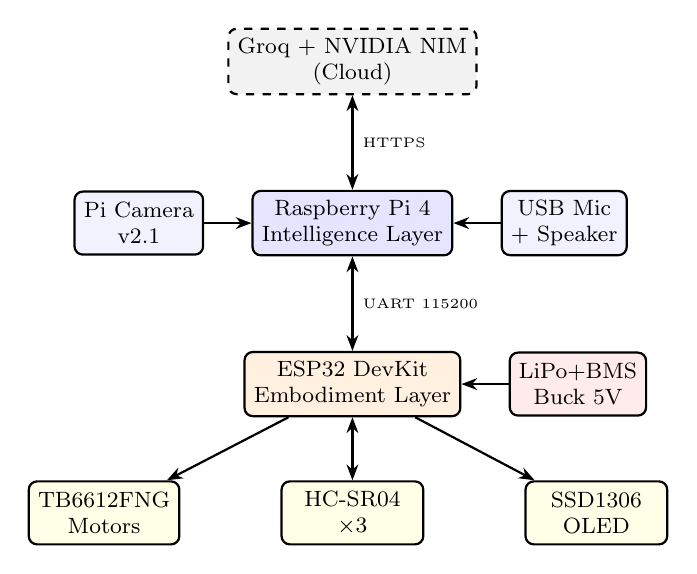
\begin{tikzpicture}[
  comp/.style={draw, thick, rounded corners=3pt, minimum height=0.8cm,
               minimum width=2.4cm, align=center, font=\footnotesize},
  bus/.style={draw, thick, -{Stealth[length=2mm]}},
  dbus/.style={draw, thick, {Stealth[length=2mm]}-{Stealth[length=2mm]}},
  node distance=0.6cm and 1.0cm
]
% Cloud
\node[comp, fill=gray!10, dashed] (cloud) {Groq + NVIDIA NIM\\(Cloud)};
% Pi
\node[comp, fill=blue!10, below=1.2cm of cloud] (pi) {Raspberry Pi 4\\Intelligence Layer};
\node[comp, fill=blue!5, left=0.6cm of pi, minimum width=1.5cm] (cam) {Pi Camera\\v2.1};
\node[comp, fill=blue!5, right=0.6cm of pi, minimum width=1.5cm] (mic) {USB Mic\\+ Speaker};
% ESP32
\node[comp, fill=orange!12, below=1.2cm of pi] (esp) {ESP32 DevKit\\Embodiment Layer};
% Peripherals
\node[comp, fill=yellow!10, below left=0.8cm and 0.8cm of esp, minimum width=1.8cm] (motor) {TB6612FNG\\Motors};
\node[comp, fill=yellow!10, below=0.8cm of esp, minimum width=1.8cm] (sensor) {HC-SR04\\$\times$3};
\node[comp, fill=yellow!10, below right=0.8cm and 0.8cm of esp, minimum width=1.8cm] (oled) {SSD1306\\OLED};
% Power
\node[comp, fill=red!8, right=0.6cm of esp, minimum width=1.5cm] (pwr) {LiPo+BMS\\Buck 5V};
% Connections
\draw[dbus] (pi) -- node[right, font=\tiny]{HTTPS} (cloud);
\draw[dbus] (pi) -- node[right, font=\tiny]{UART 115200} (esp);
\draw[bus] (cam) -- (pi);
\draw[bus] (mic) -- (pi);
\draw[bus] (esp) -- (motor);
\draw[dbus] (esp) -- (sensor);
\draw[bus] (esp) -- (oled);
\draw[bus] (pwr) -- (esp);
\end{tikzpicture}
\caption[Hardware interconnection block diagram: cloud, edge, and device tiers]{\textbf{Hardware interconnection block diagram: cloud, edge, and device tiers.}}
\label{fig:hw_block}
\end{figure}

%-------------------------------------------------------------------
\subsection{Design Constraints}
\label{subsec:design_constraints}

\begin{description}[style=nextline]
  \item[Structured Commands Only] The intelligence layer shall issue motor intents exclusively as single-line JSON objects with \textit{action} and \textit{speed}. Free-form natural language shall not be sent directly to motor routines~\cite{vemprala2024chatgpt}.

  \item[Validation Before Motion] No LLM output shall reach GPIO/PWM without passing through the validator aligned with affordance-grounding practice~\cite{ahn2022saycan,huang2023grounded}.

  \item[Bounded Action Space] The legal action set shall remain finite and enumerated in both firmware expectations and Python configuration to prevent undefined behaviours.

  \item[Graceful Degradation] Loss of cloud connectivity or Pi process failure shall not imply undefined motion: firmware falls back to AUTO\_MODE and avoidance thresholds.

  \item[Observability] Serial logging on the Pi shall record cycles, errors, and safe-stop events sufficient for debugging demonstration and safety review.

  \item[Configurability Without Reflash (Pi)] Serial baud, model name, loop interval, and timeouts shall be adjustable via configuration or environment where feasible without rebuilding firmware.
\end{description}

%-------------------------------------------------------------------
\section{Summary}
\label{sec:ch3summary}

This chapter presented the Software Requirement Specification for KANDA. The product perspective separated the ESP32 embodiment layer from the Raspberry Pi intelligence layer and identified external dependencies (Groq and NVIDIA NIM APIs, UART, power). Section~\ref{subsec:alignment} formalised the dual-service model selection and a three-layer \textit{alignment} strategy: specification (prompt), decoding (temperature and JSON contract), and runtime validation before actuation. Ten product functions covered sensing, telemetry, prompting, inference, validation, actuation, display, dual-mode operation, and shutdown behaviour. Four user classes were defined from operator to maintainer. Constraints addressed environment, language, network, credentials, electrical interfacing, and stochastic LLM latency. Fifteen functional requirements, seven performance targets aligned with implementation constants, software and hardware dependency tables, and six design constraints formalised the contract for subsequent design chapters. Grounding and validation requirements~\cite{ahn2022saycan,huang2023grounded,vemprala2024chatgpt} are central to DC-01 and DC-02 and underpin the high-level architecture in Chapter~4.

% ================================================================
%  Chapter 4 — High Level Design (KANDA)
%  Knowledge-driven Autonomous Navigation and Decision-making Agent
% ================================================================
\chapter{High Level Design}
\label{ch:hld}

This chapter explains how we designed KANDA to solve the problems from Chapter 1 while meeting the requirements from Chapter 3. Rather than start with formal specifications, we describe the real design choices and their rationale. The ESP32 handles time-critical sensing and motor control. The Raspberry Pi handles slower language-model tasks. Safety comes from three independent validation layers that check every command before motors run. We learned early that language models produce garbage sometimes, and you don't want that reaching the motors.

%-------------------------------------------------------------------
\section{Design Considerations}
\label{sec:design}

%-------------------------------------------------------------------
\subsection{General Considerations}
\label{subsec:general}

The following considerations shaped the high-level design of KANDA:

\textbf{Safety before motion:} Language models sometimes produce invalid output. Malformed JSON, made-up action names, speed values outside the valid range. Raw LLM output cannot go directly to motors. Every command must pass strict checks. Is it valid JSON? Is the action in the whitelist? Is the speed between 0 and 255? If any check fails, the robot stops.

\textbf{Layered architecture:} All components organize into independent layers. The bottom layer handles raw sensing and motor control (ESP32). The middle layer manages message passing and validation (Raspberry Pi). The top layer does reasoning (Groq, NVIDIA NIM). Each layer has a narrow interface: telemetry lines and JSON lines only. This makes debugging easier because you know where to look when something breaks.

\textbf{Timing mismatch:} The ESP32 samples sensors every 100 milliseconds. Cloud API calls take 1.5 to 4 seconds. Waiting for every cloud response would freeze the robot. Instead, the ESP32 runs local obstacle-avoidance logic independently. When the Pi goes silent (network lag or API timeout), the ESP32 avoids obstacles on its own. Not intelligent, but safe.

\textbf{Structured commands:} Instead of sending natural language to the firmware ("move forward carefully"), we send only JSON with two fields: \texttt{action} (must be one of seven words) and \texttt{speed} (must be 0--255). This way the firmware parser is dead simple and cannot be confused.

\textbf{Observability:} The OLED screen shows the robot's current state (listening, thinking, acting, searching). You can watch the robot without opening a terminal. The Pi logs all events as well. This combination saved countless debugging hours.

\textbf{Graceful degradation:} Loss of Wi-Fi, API downtime, or Pi crashes don't freeze the robot. The firmware detects silence from the Pi and switches to obstacle-avoidance mode. Not smart, but the robot stays alive.

%-------------------------------------------------------------------
\subsection{Development Methods}
\label{subsec:dev_methods}

KANDA was built incrementally: each phase works on its own before we added the next layer.

\begin{description}[nosep]
  \item[Phase 1, Foundations:] Read papers, sketch requirements, design the basic architecture (Chapters 1-3). Nothing physical yet.
  
  \item[Phase 2, Embodiment layer:] Get the ESP32 working: read ultrasonic sensors, drive motors via the H-bridge, display status on the OLED. By itself, it could avoid obstacles. No Pi, no AI, just firmware. This baseline took longer than expected because voltage dividers and sensor crosstalk are tricky.
  
  \item[Phase 3, Intelligence layer:] Add the Raspberry Pi running Python, connect to Groq (text) and NVIDIA NIM (vision), build prompts, send JSON commands to the ESP32. The firmware gets an AI\_MODE for good commands and an AUTO\_MODE fallback when the Pi is silent. The 3-second timeout proved critical for safety.
  
  \item[Phase 4, Multimodal agent:] Add camera, microphone, wake-word detection, text-to-speech, Telegram bot, and a 7-state event machine. The OLED gets animated faces. The Pi understands images and voice. This phase focuses on integration. ReAct search with semantic memory prevents revisiting areas.
\end{description}

%-------------------------------------------------------------------
\section{Architectural Strategies}
\label{sec:arch_strat}

%-------------------------------------------------------------------
\subsection{Programming Language and Runtime Selection}
\label{subsec:lang}

\textbf{Arduino-compatible C++} targets the ESP32 firmware: direct register and peripheral access, deterministic sampling intervals, mature motor-control patterns, and small binary size~\cite{espressif2023esp32}.

\textbf{Python~3} targets the Raspberry Pi intelligence layer: \texttt{pyserial} for UART communication, and fast iteration on reasoning. The system uses two cloud APIs: Groq Llama 3.3 70B for text reasoning and motion planning, and NVIDIA NIM Llama 3.2 11B Vision for visual scene understanding. We use \texttt{openWakeWord} (offline, no API) for wake detection, Google Text-to-Speech (free, no key) for voice output, and \texttt{picamera2} for image capture.

\textbf{JSON line protocol} over UART at 115,200 baud provides human-readable debugging, explicit message boundaries (newline-terminated lines), and straightforward parsing on both ends without custom framing beyond newline delimiters.

%-------------------------------------------------------------------
\subsection{Future Extensions}
\label{subsec:future}

Planned extensions beyond the baseline include on-device telemetry buffering, SLAM integration, depth sensors, and local-model experiments (Gemma 2B). All future work maintains the validation layer before actuation~\cite{huang2023grounded}.

%-------------------------------------------------------------------
\subsection{Safety Validation Pipeline}
\label{subsec:safety_pipeline}

A central design principle is \textbf{defence-in-depth}: no single layer alone protects the physical plant. Figure~\ref{fig:safety_pipeline} illustrates the three-layer safety pipeline that intercepts every command between the LLM and the motors.

\begin{figure}[H]
\centering
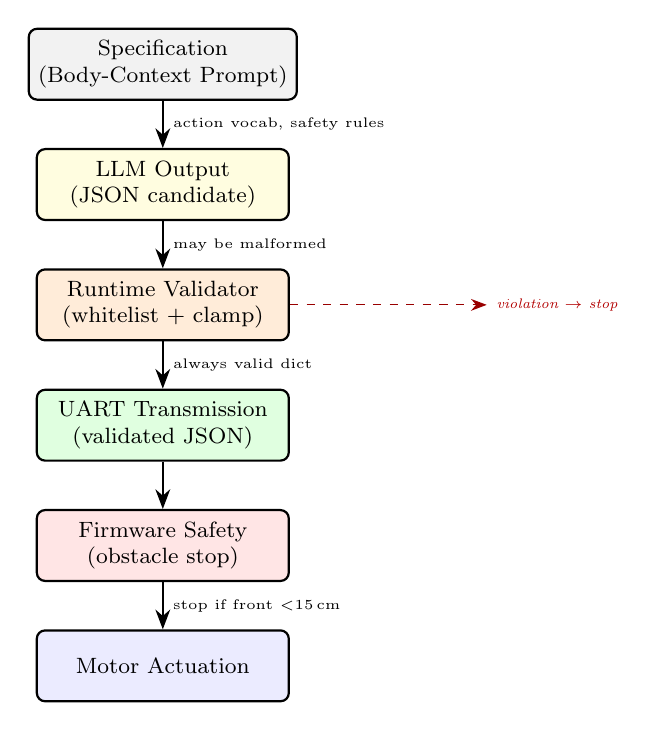
\begin{tikzpicture}[
  block/.style={draw, thick, rounded corners=3pt, minimum height=0.9cm,
                minimum width=3.2cm, align=center, font=\footnotesize},
  arr/.style={-{Stealth[length=2.5mm]}, thick},
  node distance=0.6cm
]
\node[block, fill=gray!10] (prompt) {Specification\\(Body-Context Prompt)};
\node[block, fill=yellow!12, below=of prompt] (llmout) {LLM Output\\(JSON candidate)};
\node[block, fill=orange!15, below=of llmout] (validator) {Runtime Validator\\(whitelist + clamp)};
\node[block, fill=green!12, below=of validator] (uart) {UART Transmission\\(validated JSON)};
\node[block, fill=red!10, below=of uart] (firmware) {Firmware Safety\\(obstacle stop)};
\node[block, fill=blue!8, below=of firmware] (motors) {Motor Actuation};

\draw[arr] (prompt) -- node[right, font=\tiny]{action vocab, safety rules} (llmout);
\draw[arr] (llmout) -- node[right, font=\tiny]{may be malformed} (validator);
\draw[arr] (validator) -- node[right, font=\tiny]{always valid dict} (uart);
\draw[arr] (uart) -- (firmware);
\draw[arr] (firmware) -- node[right, font=\tiny]{stop if front $<$15\,cm} (motors);

% Rejection arrows
\node[right=2.5cm of validator, font=\tiny\itshape, text=red!70!black] (reject) {violation $\to$ stop};
\draw[-{Stealth[length=2mm]}, dashed, red!60!black] (validator.east) -- (reject.west);
\end{tikzpicture}
\caption{Three-layer safety validation pipeline: specification-level grounding in the prompt, runtime enforcement on the Pi, and device-level emergency stop in ESP32 firmware.}
\label{fig:safety_pipeline}
\end{figure}

%-------------------------------------------------------------------
\section{System Architecture}
\label{sec:sysarch}

KANDA is structured as a \textbf{three-tier logical architecture}: intelligence on the Raspberry Pi, a duplex UART link, and embodiment on the ESP32 interfacing to sensors, drivers, and display. Figure~\ref{fig:sysarch} summarises the layering.

\begin{figure}[htbp!]
\centering
\resizebox{0.92\textwidth}{!}{%
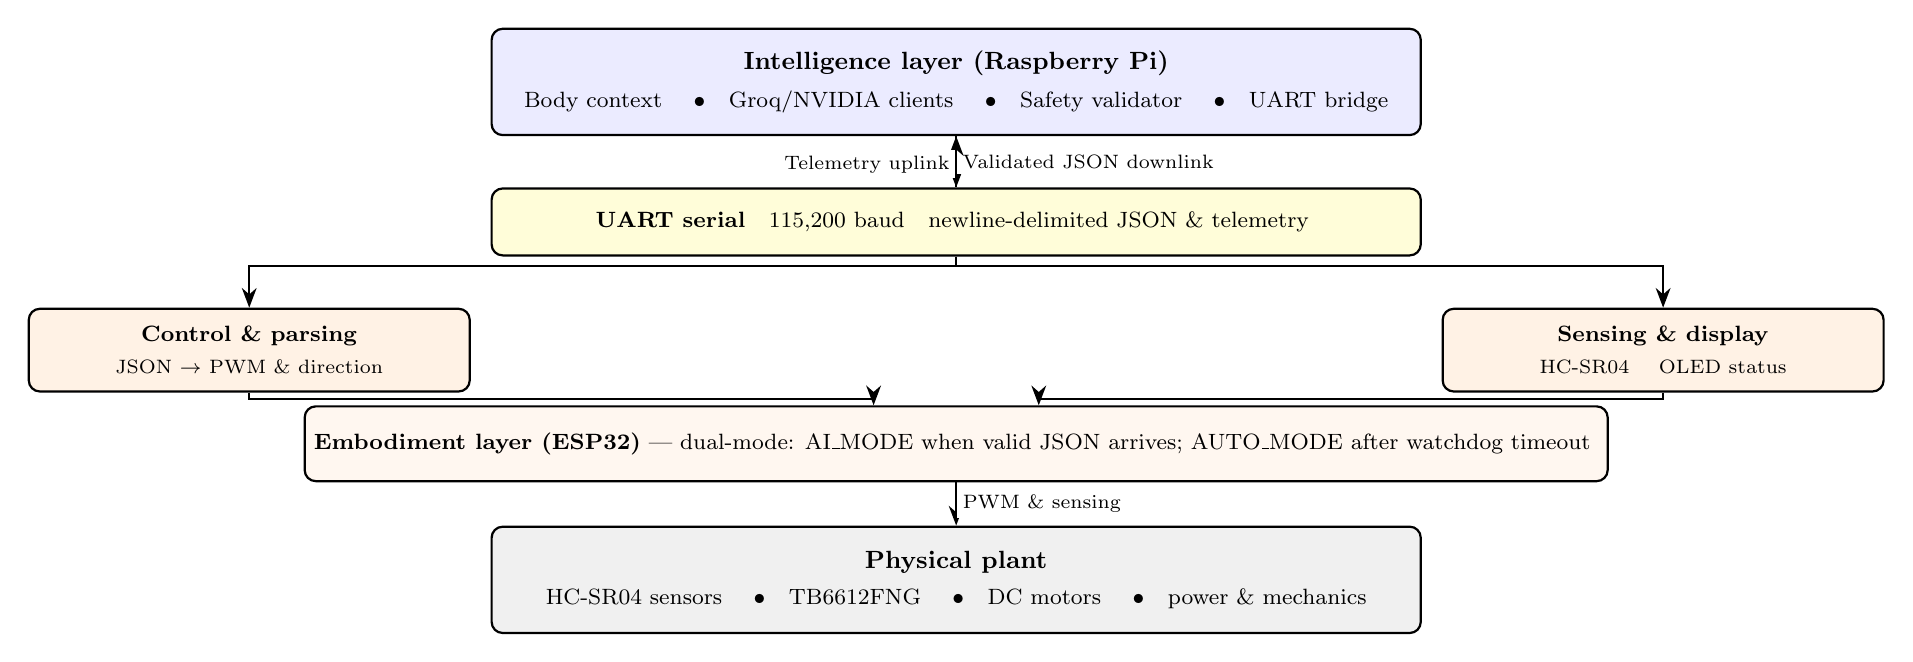
\begin{tikzpicture}[
  layer/.style={draw, thick, rounded corners=4pt, minimum width=11.8cm, minimum height=1.35cm, align=center, font=\small},
  halfbox/.style={draw, thick, rounded corners=4pt, minimum width=5.6cm, minimum height=1.05cm, align=center, font=\footnotesize},
  arr/.style={-{Stealth[length=2.5mm]}, thick},
  lbl/.style={font=\scriptsize, fill=white, inner sep=2pt},
  node distance=0.65cm
]

% Layer 1: Intelligence
\node[layer, fill=blue!8] (intel) {
  \textbf{Intelligence layer (Raspberry Pi)}\\[3pt]
  {\footnotesize Body context \quad$\bullet$\quad Groq/NVIDIA clients \quad$\bullet$\quad Safety validator \quad$\bullet$\quad UART bridge}
};

% UART link (narrow band)
\node[layer, fill=yellow!15, minimum height=0.85cm, font=\footnotesize] (uart) [below=of intel] {
  \textbf{UART serial}\quad 115,200 baud\quad newline-delimited JSON \& telemetry
};

% Embodiment: two halves
\node[halfbox, fill=orange!10, below left=0.65cm and 0.25cm of uart] (embL) {
  \textbf{Control \& parsing}\\[2pt]
  {\scriptsize JSON $\rightarrow$ PWM \& direction}
};
\node[halfbox, fill=orange!10, below right=0.65cm and 0.25cm of uart] (embR) {
  \textbf{Sensing \& display}\\[2pt]
  {\scriptsize HC-SR04 \quad OLED status}
};

\node[layer, fill=orange!6, minimum width=11.8cm, minimum height=0.95cm, font=\footnotesize] (embbar) at ($(embL.south)!0.5!(embR.south) + (0,-0.65)$) {
  \textbf{Embodiment layer (ESP32)} --- dual-mode: AI\_MODE when valid JSON arrives; AUTO\_MODE after watchdog timeout
};

% Physical
\node[layer, fill=gray!12, below=0.55cm of embbar] (phys) {
  \textbf{Physical plant}\\[2pt]
  {\footnotesize HC-SR04 sensors \quad$\bullet$\quad TB6612FNG \quad$\bullet$\quad DC motors \quad$\bullet$\quad power \& mechanics}
};

\draw[arr] (intel) -- node[lbl, right] {Validated JSON downlink} (uart);
\draw[arr] (uart) -- node[lbl, left, pos=0.45] {Telemetry uplink} (intel);

\draw[arr] (uart.south) -- ++(0,-0.12) -| (embL.north);
\draw[arr] (uart.south) -- ++(0,-0.12) -| (embR.north);

\draw[arr] (embL.south) -- ++(0,-0.08) -| (embbar.155);
\draw[arr] (embR.south) -- ++(0,-0.08) -| (embbar.25);

\draw[arr] (embbar) -- node[lbl, right] {PWM \& sensing} (phys);

\end{tikzpicture}%
}% end resizebox
\caption{High-level layered architecture of KANDA}
\label{fig:sysarch}
\end{figure}

Fig.~\ref{fig:sysarch} shows how responsibilities are split. The \textit{intelligence layer} performs hardware-aware prompting, calls Groq (text) and NVIDIA NIM (vision), validates JSON commands, and transmits safe motor intents over UART. The \textit{UART link} carries newline-terminated ASCII lines in both directions. The \textit{embodiment layer} parses commands, drives motors, samples ultrasonic sensors, refreshes the OLED, and enforces mode logic including fallback to AUTO\_MODE. The \textit{physical plant} captures sensors, actuators, and power paths documented in hardware chapters.

%-------------------------------------------------------------------
\section{Data Flow Diagrams}
\label{sec:dfd}

%-------------------------------------------------------------------
\subsection{Data Flow Diagram Level~0, Overall System}
\label{subsec:dfd0}

The Level~0 DFD places KANDA at the centre of supervision, cloud inference, and the physical deployment environment.

\begin{figure}[htbp!]
\centering
\resizebox{0.88\textwidth}{!}{%
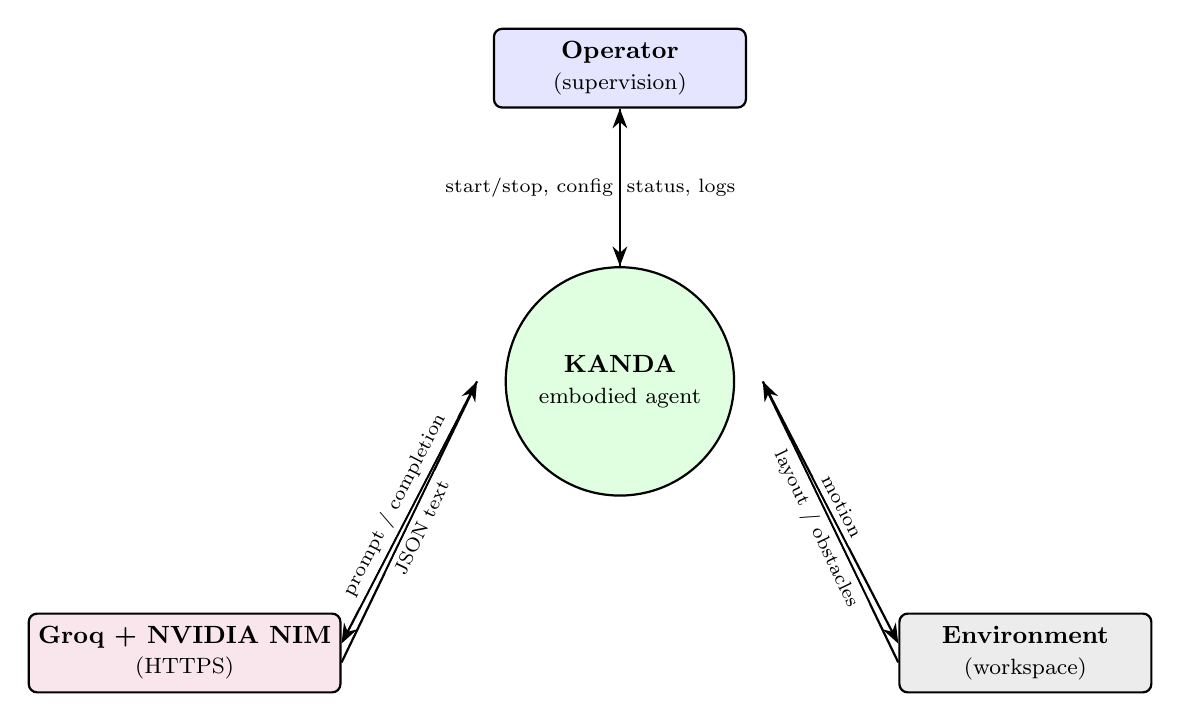
\begin{tikzpicture}[
  entity/.style={draw, thick, rectangle, rounded corners=3pt, minimum width=3.2cm, minimum height=1cm, align=center, font=\small},
  process/.style={draw, thick, circle, minimum size=2.9cm, align=center, font=\small},
  arr/.style={-{Stealth[length=2.5mm]}, thick},
  lbl/.style={font=\scriptsize, fill=white, inner sep=2pt},
  node distance=1.4cm
]

\node[entity, fill=blue!10] (op) {\textbf{Operator}\\{\footnotesize (supervision)}};

\node[process, fill=green!12, below=2cm of op] (sys) {\textbf{KANDA}\\{\footnotesize embodied agent}};

\node[entity, fill=purple!10, below left=1.9cm and 2.5cm of sys] (gem) {\textbf{Groq + NVIDIA NIM}\\{\footnotesize (HTTPS)}};

\node[entity, fill=gray!15, below right=1.9cm and 2.5cm of sys] (env) {\textbf{Environment}\\{\footnotesize (workspace)}};

\draw[arr] (op) -- node[lbl, left] {start/stop, config} (sys);
\draw[arr] (sys) -- node[lbl, right] {status, logs} (op);

\draw[arr] ([xshift=-0.35cm]sys.west) -- node[lbl, above, sloped] {prompt / completion} ([yshift=0.12cm]gem.east);
\draw[arr] ([yshift=-0.12cm]gem.east) -- node[lbl, below, sloped] {JSON text} ([xshift=-0.35cm]sys.west);

\draw[arr] ([xshift=0.35cm]sys.east) -- node[lbl, above, sloped] {motion} ([yshift=0.12cm]env.west);
\draw[arr] ([yshift=-0.12cm]env.west) -- node[lbl, below, sloped] {layout / obstacles} ([xshift=0.35cm]sys.east);

\end{tikzpicture}%
}% end resizebox
\caption{Data flow diagram Level~0, overall system}
\label{fig:dfd0}
\end{figure}

Fig.~\ref{fig:dfd0} abstracts KANDA as a single process. The \textit{operator} starts or stops runs and may adjust configuration while receiving status and logs. The system exchanges HTTPS messages with \textit{Groq and NVIDIA NIM}: prompts ascend and structured completions descend. Interaction with the \textit{environment} captures that motion changes the scene layout---including obstacle distances reflected indirectly through onboard sensing inside the system boundary.

%-------------------------------------------------------------------
\subsection{Data Flow Diagram Level~1, Embodiment and Intelligence}
\label{subsec:dfd1}

The Level~1 DFD decomposes KANDA into two cooperating sub-systems linked by the UART channel.

\begin{figure}[htbp!]
\centering
\resizebox{0.94\textwidth}{!}{%
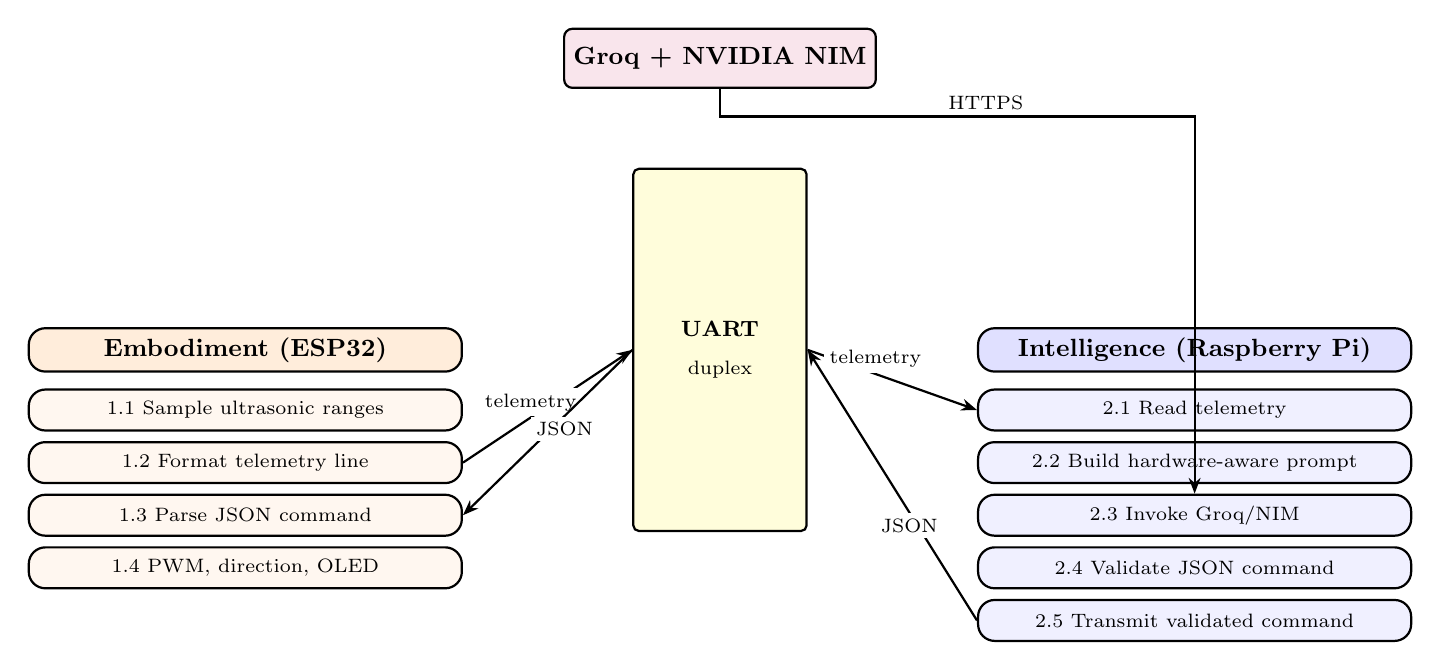
\begin{tikzpicture}[
  entity/.style={draw, thick, rectangle, rounded corners=3pt, minimum width=3cm, minimum height=0.75cm, align=center, font=\small, fill=purple!10},
  process/.style={draw, thick, rectangle, rounded corners=6pt, minimum width=5.4cm, minimum height=0.52cm, align=center, font=\small},
  chan/.style={draw, thick, rectangle, rounded corners=2pt, minimum width=2.2cm, minimum height=4.6cm, align=center, font=\footnotesize, fill=yellow!14},
  arr/.style={-{Stealth[length=2mm]}, thick},
  lbl/.style={font=\scriptsize, fill=white, inner sep=2pt},
  node distance=0.32cm
]

\node[entity] (gem) {\textbf{Groq + NVIDIA NIM}};

% UART channel (centre spine)
\node[chan, below=1cm of gem] (uart) {\textbf{UART}\\[4pt]{\scriptsize duplex}};

% LEFT: Embodiment column (ESP32)
\node[process, fill=orange!14, font=\small\bfseries, left=2.15cm of uart, anchor=east, minimum width=5.5cm] (e0) {Embodiment (ESP32)};
\node[process, fill=orange!6, below=0.2cm of e0, font=\scriptsize, minimum width=5.5cm] (e1) {1.1 Sample ultrasonic ranges};
\node[process, fill=orange!6, below=0.12cm of e1, font=\scriptsize, minimum width=5.5cm] (e2) {1.2 Format telemetry line};
\node[process, fill=orange!6, below=0.12cm of e2, font=\scriptsize, minimum width=5.5cm] (e3) {1.3 Parse JSON command};
\node[process, fill=orange!6, below=0.12cm of e3, font=\scriptsize, minimum width=5.5cm] (e4) {1.4 PWM, direction, OLED};

% RIGHT: Intelligence column (Pi)
\node[process, fill=blue!12, font=\small\bfseries, right=2.15cm of uart, anchor=west, minimum width=5.5cm] (i0) {Intelligence (Raspberry Pi)};
\node[process, fill=blue!6, below=0.2cm of i0, font=\scriptsize, minimum width=5.5cm] (i1) {2.1 Read telemetry};
\node[process, fill=blue!6, below=0.12cm of i1, font=\scriptsize, minimum width=5.5cm] (i2) {2.2 Build hardware-aware prompt};
\node[process, fill=blue!6, below=0.12cm of i2, font=\scriptsize, minimum width=5.5cm] (i3) {2.3 Invoke Groq/NIM};
\node[process, fill=blue!6, below=0.12cm of i3, font=\scriptsize, minimum width=5.5cm] (i4) {2.4 Validate JSON command};
\node[process, fill=blue!6, below=0.12cm of i4, font=\scriptsize, minimum width=5.5cm] (i5) {2.5 Transmit validated command};

% Cloud APIs to intelligence (HTTPS inference)
\draw[arr] (gem.south) -- +(0,-0.35) -| node[lbl, pos=0.28, above] {HTTPS} (i3.north);

% Telemetry uplink: embodiment -> uart -> intelligence
\draw[arr] (e2.east) -- node[lbl, above, pos=0.4] {telemetry} (uart.west);

\draw[arr] (uart.east) -- node[lbl, above, pos=0.4] {telemetry} (i1.west);

% Command downlink: intelligence -> uart -> embodiment
\draw[arr] (i5.west) -- node[lbl, below, pos=0.4] {JSON} (uart.east);

\draw[arr] (uart.west) -- node[lbl, below, pos=0.4] {JSON} (e3.east);

\end{tikzpicture}%
}% end resizebox
\caption{Data flow diagram Level~1, embodiment and intelligence sub-systems}
\label{fig:dfd1}
\end{figure}

Fig.~\ref{fig:dfd1} separates real-time embodiment (left) from asynchronous intelligence (right). Telemetry formatted on the ESP32 flows upward to the Raspberry Pi; validated JSON commands flow downward after prompt construction, cloud inference, and validation. HTTPS exchanges with Groq and NVIDIA NIM attach to the intelligence column (expanded at Level~2).

%-------------------------------------------------------------------
\subsection{Data Flow Diagram Level~2, Intelligence Pipeline}
\label{subsec:dfd2_intel}

\begin{figure}[htbp!]
\centering
\resizebox{0.82\textwidth}{!}{%
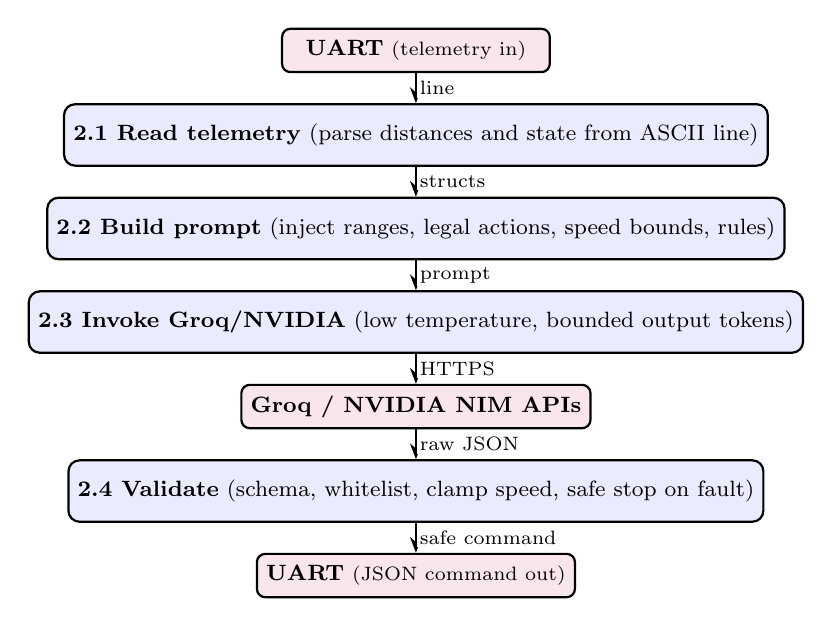
\begin{tikzpicture}[
  proc/.style={draw, thick, rectangle, rounded corners=4pt, minimum width=8.8cm, minimum height=0.78cm, align=center, font=\footnotesize, fill=blue!8},
  ext/.style={draw, thick, rectangle, rounded corners=3pt, minimum width=3.4cm, minimum height=0.55cm, align=center, font=\footnotesize, fill=purple!10},
  arr/.style={-{Stealth[length=2mm]}, thick},
  lbl/.style={font=\scriptsize, fill=white, inner sep=1pt},
  node distance=0.38cm
]

\node[ext] (uartin) {\textbf{UART} {\scriptsize (telemetry in)}};

\node[proc, below=of uartin] (p1) {\textbf{2.1 Read telemetry} (parse distances and state from ASCII line)};

\node[proc, below=of p1] (p2) {\textbf{2.2 Build prompt} (inject ranges, legal actions, speed bounds, rules)};

\node[proc, below=of p2] (p3) {\textbf{2.3 Invoke Groq/NVIDIA} (low temperature, bounded output tokens)};

\node[ext, below=of p3] (gem) {\textbf{Groq / NVIDIA NIM APIs}};

\node[proc, below=of gem] (p4) {\textbf{2.4 Validate} (schema, whitelist, clamp speed, safe stop on fault)};

\node[ext, below=of p4] (uartout) {\textbf{UART} {\scriptsize (JSON command out)}};

\draw[arr] (uartin) -- node[lbl, right] {line} (p1);
\draw[arr] (p1) -- node[lbl, right] {structs} (p2);
\draw[arr] (p2) -- node[lbl, right] {prompt} (p3);
\draw[arr] (p3) -- node[lbl, right] {HTTPS} (gem);
\draw[arr] (gem) -- node[lbl, right] {raw JSON} (p4);
\draw[arr] (p4) -- node[lbl, right] {safe command} (uartout);

\end{tikzpicture}%
}% end resizebox
\caption{Data flow diagram Level~2, intelligence pipeline on the Raspberry Pi}
\label{fig:dfd2a}
\end{figure}

Fig.~\ref{fig:dfd2a} details the Pi-side pipeline implemented by \path|vision_module/main.py| and companion modules: telemetry ingestion, hardware-aware prompt construction, Groq/NVIDIA invocation, validation, and transmission of a single safe JSON line per cycle.

%-------------------------------------------------------------------
\subsection{Data Flow Diagram Level~2, Embodiment Pipeline}
\label{subsec:dfd2_emb}

\begin{figure}[htbp!]
\centering
\resizebox{0.82\textwidth}{!}{%
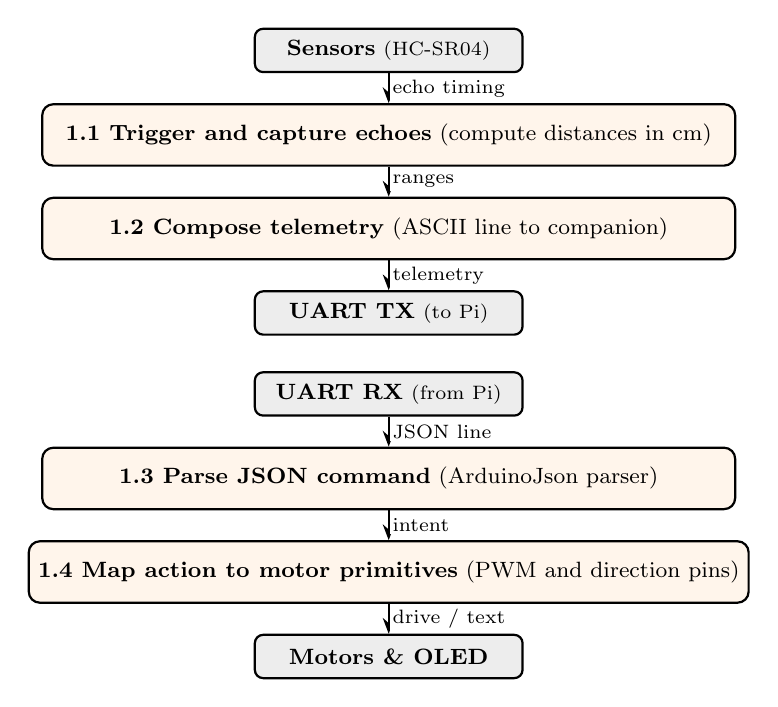
\begin{tikzpicture}[
  proc/.style={draw, thick, rectangle, rounded corners=4pt, minimum width=8.8cm, minimum height=0.78cm, align=center, font=\footnotesize, fill=orange!8},
  ext/.style={draw, thick, rectangle, rounded corners=3pt, minimum width=3.4cm, minimum height=0.55cm, align=center, font=\footnotesize, fill=gray!14},
  arr/.style={-{Stealth[length=2mm]}, thick},
  lbl/.style={font=\scriptsize, fill=white, inner sep=1pt},
  node distance=0.38cm
]

\node[ext] (sns) {\textbf{Sensors} {\scriptsize (HC-SR04)}};

\node[proc, below=of sns] (p1) {\textbf{1.1 Trigger and capture echoes} (compute distances in cm)};

\node[proc, below=of p1] (p2) {\textbf{1.2 Compose telemetry} (ASCII line to companion)};

\node[ext, below=of p2] (uartup) {\textbf{UART TX} {\scriptsize (to Pi)}};

\node[ext, below=0.45cm of uartup] (uartdn) {\textbf{UART RX} {\scriptsize (from Pi)}};

\node[proc, below=of uartdn] (p3) {\textbf{1.3 Parse JSON command} (ArduinoJson parser)};

\node[proc, below=of p3] (p4) {\textbf{1.4 Map action to motor primitives} (PWM and direction pins)};

\node[ext, below=of p4] (mot) {\textbf{Motors \& OLED}};

\draw[arr] (sns) -- node[lbl, right] {echo timing} (p1);
\draw[arr] (p1) -- node[lbl, right] {ranges} (p2);
\draw[arr] (p2) -- node[lbl, right] {telemetry} (uartup);

\draw[arr] (uartdn) -- node[lbl, right] {JSON line} (p3);
\draw[arr] (p3) -- node[lbl, right] {intent} (p4);
\draw[arr] (p4) -- node[lbl, right] {drive / text} (mot);

\end{tikzpicture}%
}% end resizebox
\caption{Data flow diagram Level~2, embodiment pipeline on the ESP32}
\label{fig:dfd2b}
\end{figure}

Fig.~\ref{fig:dfd2b} expands embodiment-side processing: ranging, telemetry uplink, inbound JSON parsing, mapping discrete actions to TB6612FNG outputs, and operator-visible OLED updates. Watchdog and AUTO\_MODE transitions are policy logic around these flows.

%-------------------------------------------------------------------
\section{Summary}
\label{sec:ch4summary}

This chapter presented the high-level design of KANDA. Design considerations emphasised validation before actuation~\cite{huang2023grounded}, affordance-grounded command formats~\cite{ahn2022saycan}, layered embodied structure~\cite{brooks1986robust}, and resilience to stochastic cloud latency~\cite{vemprala2024chatgpt}. Development followed phased delivery from embodiment to intelligence, with a documented path toward multimodal extensions~\cite{zeng2023socratic,wu2023tidybot}.

Architectural strategies justified C++ on the ESP32 and Python on the Raspberry Pi, linked by a newline-delimited JSON and telemetry UART protocol~\cite{espressif2023esp32}. Figure~\ref{fig:sysarch} summarised the intelligence, UART, embodiment, and physical tiers. Data flow diagrams at Level~0 (\ref{fig:dfd0}), Level~1 (\ref{fig:dfd1}), and Level~2 (\ref{fig:dfd2a}, \ref{fig:dfd2b}) traced information from sensors and cloud inference to motor outputs. Chapter~5 refines these sub-systems into detailed module-level design aligned with the implementation directories.

% ================================================================
%  Chapter 5 — Detailed Design (KANDA)
%  Knowledge-driven Autonomous Navigation and Decision-making Agent
% ================================================================
\chapter{Detailed Design}
\label{ch:detail}

This chapter presents the detailed design of \textbf{Knowledge-driven Autonomous Navigation and Decision-making Agent (KANDA)} at module and component level. It builds on the high-level architecture and data flows in Chapter~\ref{ch:hld}: overview diagrams, use cases, deployment components, a structure chart for the Python orchestrator, an activity view of one control cycle, and descriptions of each software module together with the embodiment firmware running on the ESP32.

%-------------------------------------------------------------------
\section{High-Level Design Overview}
\label{sec:hld_overview}

The deployment comprises a Raspberry Pi running the Python package tree \texttt{ai\_layer/}, an ESP32 running Arduino-compatible firmware under \texttt{firmware/phase2\_obstacle\_avoidance/}, a duplex UART link, and HTTPS access to Google Gemini (default model \texttt{gemini-2.5-flash}). Figure~\ref{fig:hld_overview} summarises the principal deployable blocks.

\begin{figure}[htbp!]
\centering
\resizebox{0.9\textwidth}{!}{%
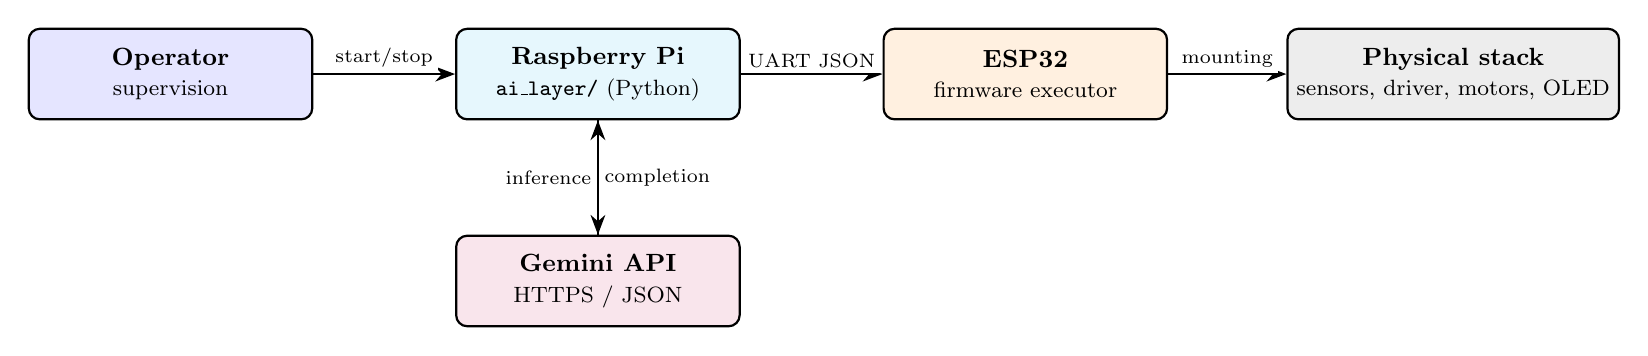
\begin{tikzpicture}[
  block/.style={draw, thick, rounded corners=4pt, minimum width=3.6cm, minimum height=1.15cm, align=center, font=\small},
  arr/.style={-{Stealth[length=2.5mm]}, thick},
  darr/.style={-{Stealth[length=2.5mm]}, thick, densely dashed},
  lbl/.style={font=\scriptsize, fill=white, inner sep=2pt},
  node distance=1.1cm
]

\node[block, fill=blue!10] (op) {\textbf{Operator}\\{\footnotesize supervision}};

\node[block, fill=cyan!10, right=1.8cm of op] (pi) {\textbf{Raspberry Pi}\\{\footnotesize \texttt{ai\_layer/} (Python)}};

\node[block, fill=orange!12, right=1.8cm of pi] (esp) {\textbf{ESP32}\\{\footnotesize firmware executor}};

\node[block, fill=purple!10, below=1.45cm of pi] (gem) {\textbf{Gemini API}\\{\footnotesize HTTPS / JSON}};

\node[block, fill=gray!14, right=1.5cm of esp] (phys) {\textbf{Physical stack}\\{\footnotesize sensors, driver, motors, OLED}};

\draw[arr] (op) -- node[lbl, above] {start/stop} (pi);
\draw[arr] (pi) -- node[lbl, above] {UART JSON} (esp);
\draw[arr] (esp) -- node[lbl, above] {mounting} (phys);
\draw[arr] (pi.south) -- node[lbl, left] {inference} (gem.north);
\draw[arr] (gem.north) -- node[lbl, right] {completion} (pi.south);

\end{tikzpicture}%
}% end resizebox
\caption{High-level deployable blocks of KANDA}
\label{fig:hld_overview}
\end{figure}

Fig.~\ref{fig:hld_overview} shows how the operator interacts with the intelligence layer on the Pi, how the Pi exchanges newline-terminated JSON and telemetry with the ESP32 over UART, how the ESP32 connects to the physical stack, and how the Pi calls the Gemini API over the network.

%-------------------------------------------------------------------
\section{Low-Level Design Overview}
\label{sec:lld_overview}

The Python intelligence layer is organised into configuration, serial I/O, prompt construction, LLM access, validation, and a single orchestrator entry point. Figure~\ref{fig:lld_overview} maps files to these roles.

\begin{figure}[htbp!]
\centering
\resizebox{0.94\textwidth}{!}{%
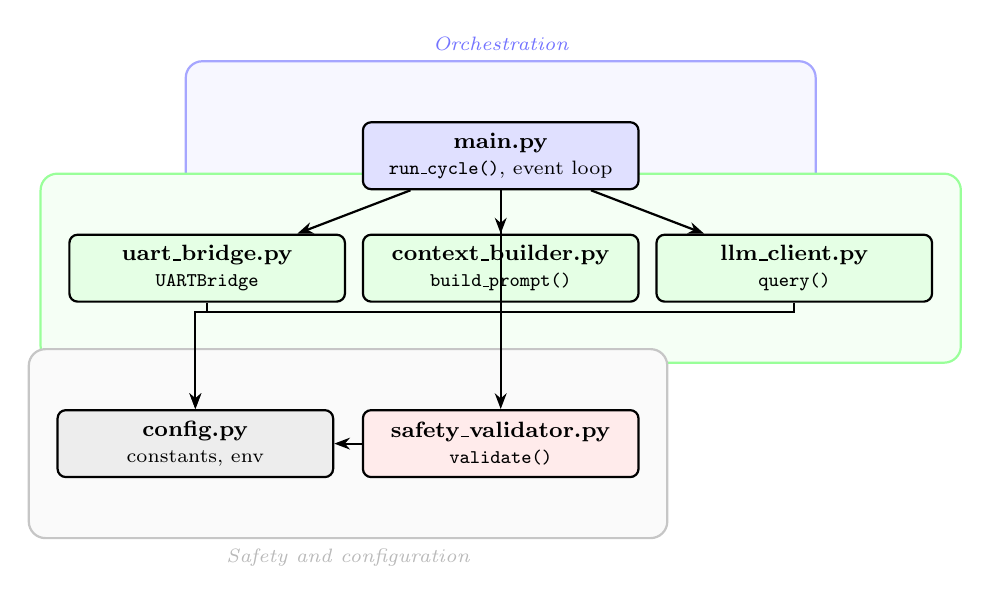
\begin{tikzpicture}[
  mod/.style={draw, thick, rounded corners=3pt, minimum width=3.5cm, minimum height=0.85cm, align=center, font=\footnotesize},
  grp/.style={draw, thick, rounded corners=6pt, minimum width=8cm, minimum height=2.4cm},
  arr/.style={-{Stealth[length=2mm]}, thick},
  lbl/.style={font=\tiny, fill=white, inner sep=1pt},
  node distance=0.45cm
]

\node[mod, fill=blue!12] (main) {\textbf{main.py}\\{\scriptsize \texttt{run\_cycle()}, event loop}};
\node[mod, fill=green!10, below left=0.55cm and 0.2cm of main] (uart) {\textbf{uart\_bridge.py}\\{\scriptsize \texttt{UARTBridge}}};
\node[mod, fill=green!10, below=0.55cm of main] (ctx) {\textbf{context\_builder.py}\\{\scriptsize \texttt{build\_prompt()}}};
\node[mod, fill=green!10, below right=0.55cm and 0.2cm of main] (llm) {\textbf{llm\_client.py}\\{\scriptsize \texttt{query()}}};

\node[mod, fill=red!8, below=1.35cm of ctx] (val) {\textbf{safety\_validator.py}\\{\scriptsize \texttt{validate()}}};
\node[mod, fill=gray!14, left=0.35cm of val] (cfg) {\textbf{config.py}\\{\scriptsize constants, env}};

\draw[arr] (main) -- (uart);
\draw[arr] (main) -- (ctx);
\draw[arr] (main) -- (llm);
\draw[arr] (main) -- (val);
\draw[arr] (llm.south) -- ++(0,-0.12) -| (cfg.north);
\draw[arr] (val.west) -- (cfg.east);
\draw[arr] (uart.south) -- ++(0,-0.12) -| (cfg.north);

\begin{scope}[on background layer]
  \node[grp, fill=blue!3, draw=blue!35, fit=(main), inner sep=10pt, label={[font=\scriptsize\itshape, text=blue!55]above:Orchestration}] {};
  \node[grp, fill=green!4, draw=green!40, fit=(uart)(ctx)(llm), inner sep=10pt, label={[font=\scriptsize\itshape, text=green!55]above:I/O and reasoning}] {};
  \node[grp, fill=gray!4, draw=gray!45, fit=(val)(cfg), inner sep=10pt, label={[font=\scriptsize\itshape, text=gray!55]below:Safety and configuration}] {};
\end{scope}

\end{tikzpicture}%
}% end resizebox
\caption{Low-level design: Python modules under \texttt{ai\_layer/}}
\label{fig:lld_overview}
\end{figure}

Fig.~\ref{fig:lld_overview} reflects the call pattern described in Section~\ref{sec:modules}: \texttt{main.py} invokes UART bridge, prompt builder, LLM client, and validator; \texttt{config.py} supplies shared limits and environment-backed settings to clients that depend on model id, serial port, and action sets.

%-------------------------------------------------------------------
\section{Use Case Diagram}
\label{sec:usecase}

Figure~\ref{fig:usecase} relates actors to the operational use cases of the deployed robot and cloud service.

\begin{figure}[htbp!]
\centering
\resizebox{0.85\textwidth}{!}{%
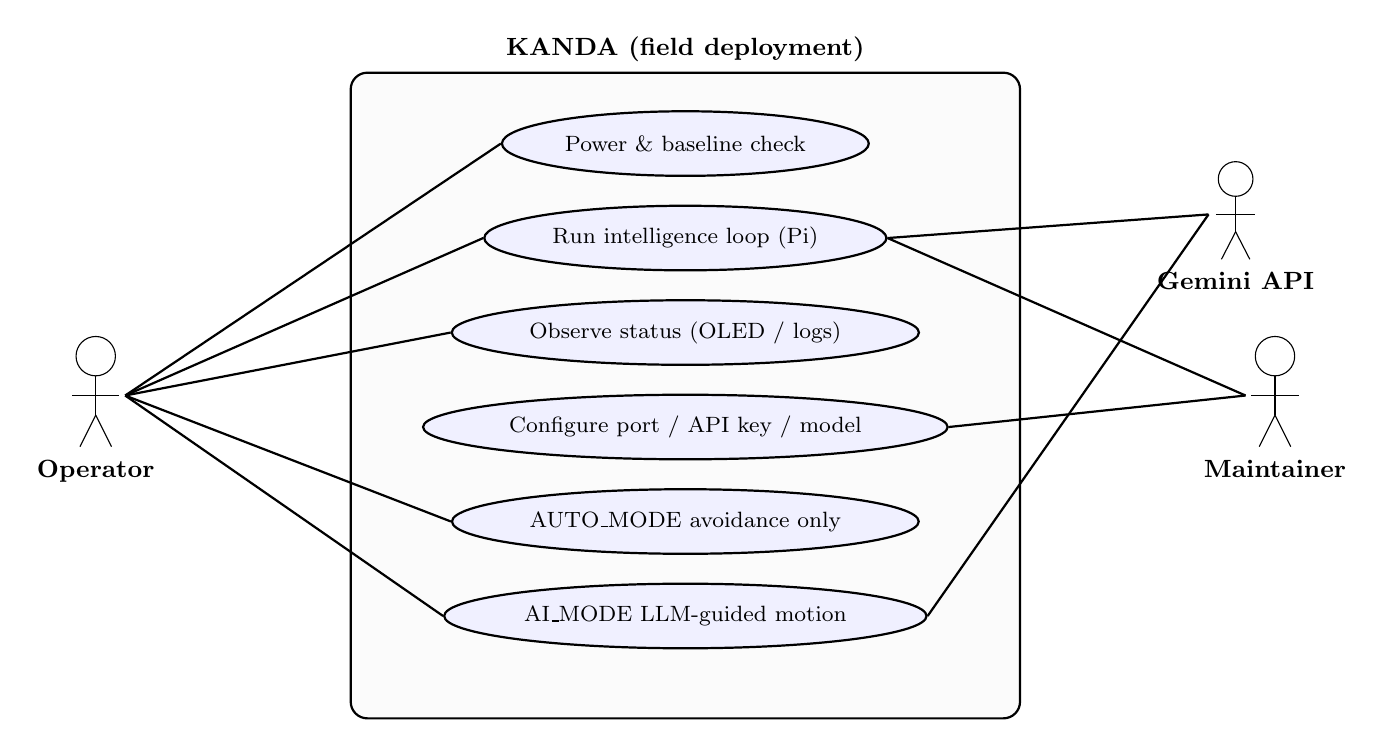
\begin{tikzpicture}[
  actor/.style={font=\small},
  uc/.style={draw, thick, ellipse, minimum width=3.6cm, minimum height=0.82cm, align=center, font=\footnotesize, fill=blue!6},
  arr/.style={-{Stealth[length=2mm]}, thick},
  sys/.style={draw, thick, rounded corners=6pt, minimum width=8.5cm, minimum height=8.2cm, fill=gray!3},
  node distance=0.45cm
]

\node[sys, label={[font=\small\bfseries]above:KANDA (field deployment)}] (boundary) {};

\node[uc] at (0, 3.2) (uc1) {Power \& baseline check};
\node[uc] at (0, 2.0) (uc2) {Run intelligence loop (Pi)};
\node[uc] at (0, 0.8) (uc3) {Observe status (OLED / logs)};
\node[uc] at (0, -0.4) (uc4) {Configure port / API key / model};
\node[uc] at (0, -1.6) (uc5) {AUTO\_MODE avoidance only};
\node[uc] at (0, -2.8) (uc6) {AI\_MODE LLM-guided motion};

\node[actor, left=3.1cm of boundary.west] (user) {};
\draw (user) ++(0,0.5) circle(0.25);
\draw (user) ++(0,0.25) -- ++(0,-0.5);
\draw (user) ++(-0.3,0) -- ++(0.6,0);
\draw (user) ++(0,-0.25) -- ++(-0.2,-0.4);
\draw (user) ++(0,-0.25) -- ++(0.2,-0.4);
\node[font=\small\bfseries, below=0.08cm] at ([yshift=-0.62cm]user) {Operator};

\node[actor, right=3.1cm of boundary.east] (dev) {};
\draw (dev) ++(0,0.5) circle(0.25);
\draw (dev) ++(0,0.25) -- ++(0,-0.5);
\draw (dev) ++(-0.3,0) -- ++(0.6,0);
\draw (dev) ++(0,-0.25) -- ++(-0.2,-0.4);
\draw (dev) ++(0,-0.25) -- ++(0.2,-0.4);
\node[font=\small\bfseries, below=0.08cm] at ([yshift=-0.62cm]dev) {Maintainer};

\node[actor, right=2.6cm of boundary.east, yshift=2.3cm] (gemact) {};
\draw (gemact) ++(0,0.45) circle(0.22);
\draw (gemact) ++(0,0.22) -- ++(0,-0.45);
\draw (gemact) ++(-0.25,0) -- ++(0.5,0);
\draw (gemact) ++(0,-0.22) -- ++(-0.18,-0.35);
\draw (gemact) ++(0,-0.22) -- ++(0.18,-0.35);
\node[font=\small\bfseries, below=0.06cm] at ([yshift=-0.55cm]gemact) {Gemini API};

\draw[thick] ([xshift=0.25cm]user.east) -- (uc1.west);
\draw[thick] ([xshift=0.25cm]user.east) -- (uc2.west);
\draw[thick] ([xshift=0.25cm]user.east) -- (uc3.west);
\draw[thick] ([xshift=0.25cm]user.east) -- (uc5.west);
\draw[thick] ([xshift=0.25cm]user.east) -- (uc6.west);

\draw[thick] ([xshift=-0.25cm]dev.west) -- (uc4.east);
\draw[thick] ([xshift=-0.25cm]dev.west) -- (uc2.east);

\draw[thick] ([xshift=-0.22cm]gemact.west) -- (uc2.east);
\draw[thick] ([xshift=-0.22cm]gemact.west) -- (uc6.east);

\end{tikzpicture}%
}% end resizebox
\caption{Use case diagram for KANDA deployment}
\label{fig:usecase}
\end{figure}

The \textit{operator} powers the platform, starts or stops the Pi process, reads the OLED, and relies on obstacle behaviour in AUTO\_MODE or guided behaviour in AI\_MODE. The \textit{maintainer} adjusts serial device paths, credentials, and model identifiers. The \textit{Gemini API} participates whenever the intelligence loop issues HTTPS inference requests.

%-------------------------------------------------------------------
\section{Component Diagram}
\label{sec:component}

Figure~\ref{fig:component} packages software onto the two compute nodes and shows external services.

\begin{figure}[htbp!]
\centering
\resizebox{0.9\textwidth}{!}{%
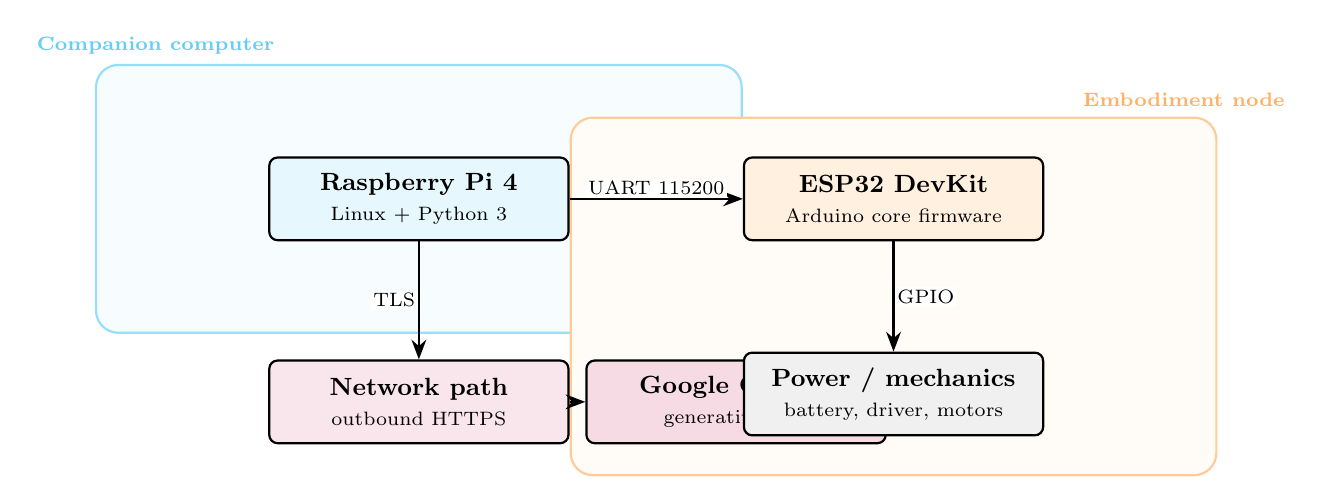
\begin{tikzpicture}[
  comp/.style={draw, thick, rounded corners=3pt, minimum width=3.8cm, minimum height=1.05cm, align=center, font=\small, fill=white},
  pkg/.style={draw, thick, rounded corners=8pt, minimum width=8.2cm, minimum height=3.4cm},
  arr/.style={-{Stealth[length=2.5mm]}, thick},
  lbl/.style={font=\scriptsize, fill=white, inner sep=1pt},
  node distance=0.75cm
]

\node[comp, fill=cyan!10] (pi) {\textbf{Raspberry Pi 4}\\{\scriptsize Linux + Python 3}};

\node[comp, fill=orange!12, right=2.2cm of pi] (esp) {\textbf{ESP32 DevKit}\\{\scriptsize Arduino core firmware}};

\node[comp, fill=purple!10, below=1.5cm of pi] (net) {\textbf{Network path}\\{\scriptsize outbound HTTPS}};

\node[comp, fill=purple!14, right=0.2cm of net] (gem) {\textbf{Google Gemini}\\{\scriptsize generative API}};

\node[comp, fill=gray!12, below=1.4cm of esp] (bat) {\textbf{Power / mechanics}\\{\scriptsize battery, driver, motors}};

\draw[arr] (pi) -- node[lbl, above] {UART 115200} (esp);
\draw[arr] (pi) -- node[lbl, left] {TLS} (net);
\draw[arr] (net) -- (gem);
\draw[arr] (esp) -- node[lbl, right] {GPIO} (bat);

\begin{scope}[on background layer]
  \node[pkg, fill=cyan!3, draw=cyan!40, fit=(pi), inner sep=14pt, label={[font=\scriptsize\bfseries, text=cyan!60]above left:Companion computer}] {};
  \node[pkg, fill=orange!3, draw=orange!40, fit=(esp)(bat), inner sep=14pt, label={[font=\scriptsize\bfseries, text=orange!60]above right:Embodiment node}] {};
\end{scope}

\end{tikzpicture}%
}% end resizebox
\caption{Component diagram: companion computer, embodiment node, and cloud API}
\label{fig:component}
\end{figure}

The Raspberry Pi component hosts the entire \texttt{ai\_layer/} tree. The ESP32 component hosts sensing, actuation, OLED rendering, and UART framing. Gemini is an external software service accessed only from the Pi.

%-------------------------------------------------------------------
\section{Structure Chart}
\label{sec:structure_chart}

Figure~\ref{fig:structure_chart} shows the static decomposition of the orchestrator and its collaborators.

\begin{figure}[htbp!]
\centering
\resizebox{0.95\textwidth}{!}{%
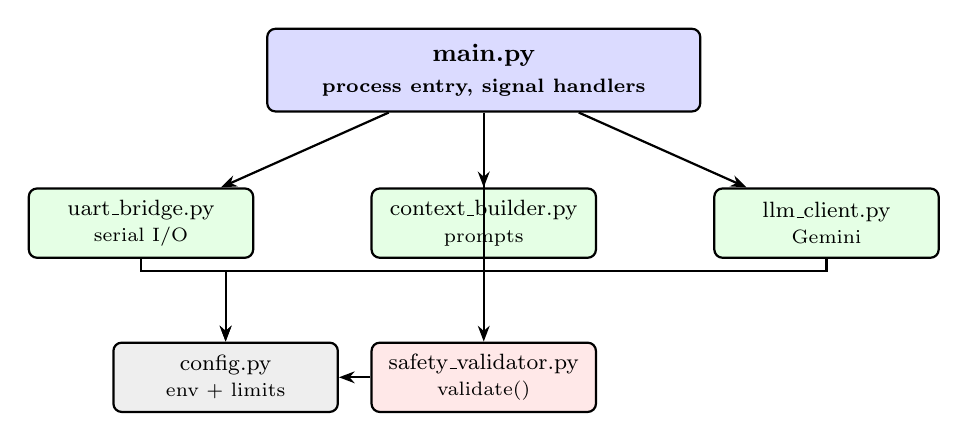
\begin{tikzpicture}[
  mod/.style={draw, thick, rounded corners=3pt, minimum width=2.85cm, minimum height=0.88cm, align=center, font=\footnotesize},
  top/.style={mod, fill=blue!14, minimum width=5.5cm, minimum height=1.05cm, font=\small\bfseries},
  arr/.style={-{Stealth[length=2mm]}, thick},
  lbl/.style={font=\tiny, fill=white, inner sep=1pt},
  node distance=0.55cm
]

\node[top] (main) {main.py\\\scriptsize process entry, signal handlers};

\node[mod, fill=green!10, below left=0.95cm and 0.15cm of main] (uart) {uart\_bridge.py\\\scriptsize serial I/O};
\node[mod, fill=green!10, below=0.95cm of main] (ctx) {context\_builder.py\\\scriptsize prompts};
\node[mod, fill=green!10, below right=0.95cm and 0.15cm of main] (llm) {llm\_client.py\\\scriptsize Gemini};

\node[mod, fill=red!9, below=1.05cm of ctx] (val) {safety\_validator.py\\\scriptsize validate()};

\node[mod, fill=gray!13, left=0.4cm of val] (cfg) {config.py\\\scriptsize env + limits};

\draw[arr] (main) -- (uart);
\draw[arr] (main) -- (ctx);
\draw[arr] (main) -- (llm);
\draw[arr] (main) -- (val);
\draw[arr] (llm.south) -- ++(0,-0.15) -| (cfg.north);
\draw[arr] (val.west) -- (cfg.east);
\draw[arr] (uart.south) -- ++(0,-0.15) -| (cfg.north);

\end{tikzpicture}%
}% end resizebox
\caption{Structure chart: intelligence layer modules}
\label{fig:structure_chart}
\end{figure}

Entry resolves in \texttt{main.py}: an infinite loop calls \texttt{run\_cycle()}, which sequences UART reads, prompt construction, Gemini inference, validation, and command transmission. Shared constants and limits live in \texttt{config.py}.

%-------------------------------------------------------------------
\section{Control Cycle Activity View}
\label{sec:activity}

Figure~\ref{fig:activity_cycle} refines the Level~2 intelligence pipeline from Chapter~\ref{ch:hld} into the conditional branches implemented in code.

\begin{figure}[htbp!]
\centering
\resizebox{0.72\textwidth}{!}{%
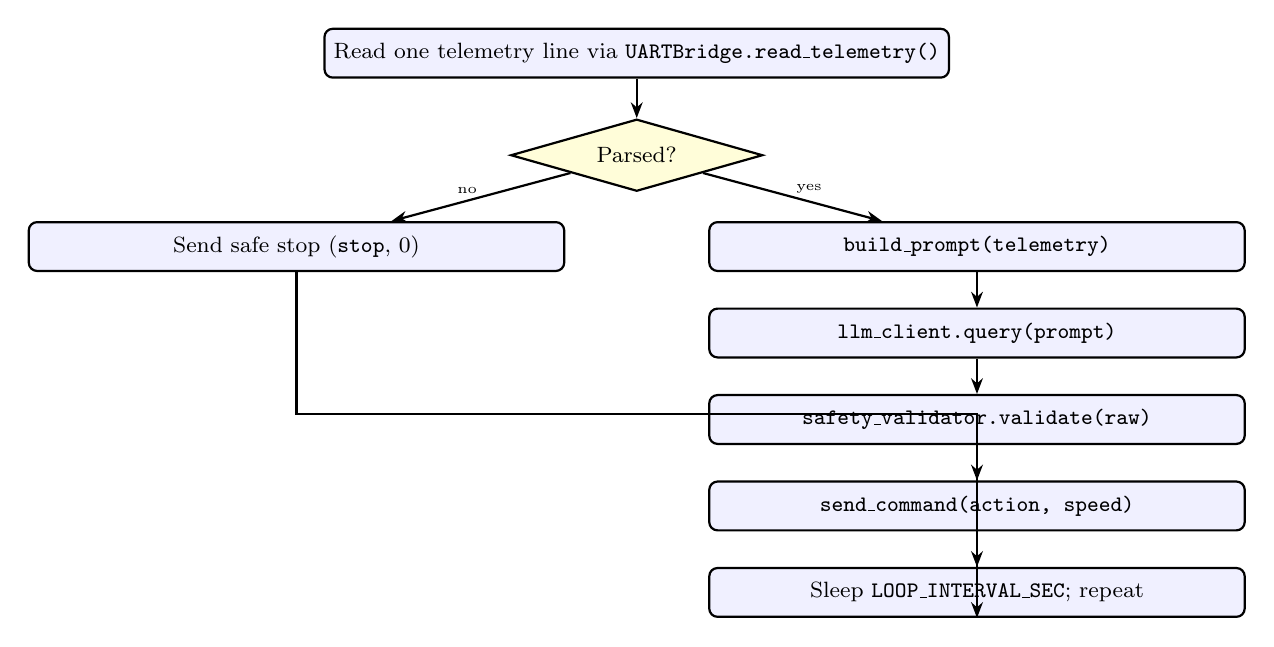
\begin{tikzpicture}[
  flowstep/.style={draw, thick, rounded corners=3pt, minimum width=6.8cm, minimum height=0.62cm, align=center, font=\footnotesize, fill=blue!6},
  dec/.style={draw, thick, diamond, aspect=2, minimum width=3.2cm, inner sep=2pt, align=center, font=\footnotesize, fill=yellow!15},
  arr/.style={-{Stealth[length=2mm]}, thick},
  lbl/.style={font=\tiny, fill=white, inner sep=1pt},
  node distance=0.42cm
]

\node[flowstep] (a) {Read one telemetry line via \texttt{UARTBridge.read\_telemetry()}};
\node[dec, below=0.5cm of a] (b) {Parsed?};
\node[flowstep, below left=0.6cm and 0.1cm of b] (c) {Send safe stop (\texttt{stop}, 0)};
\node[flowstep, below right=0.6cm and 0.1cm of b] (d) {\texttt{build\_prompt(telemetry)}};
\node[flowstep, below=0.45cm of d] (e) {\texttt{llm\_client.query(prompt)}};
\node[flowstep, below=0.45cm of e] (f) {\texttt{safety\_validator.validate(raw)}};
\node[flowstep, below=0.45cm of f] (g) {\texttt{send\_command(action, speed)}};
\node[flowstep, below=0.45cm of g] (h) {Sleep \texttt{LOOP\_INTERVAL\_SEC}; repeat};

\draw[arr] (a) -- (b);
\draw[arr] (b) -- node[lbl, above left] {no} (c);
\draw[arr] (b) -- node[lbl, above right] {yes} (d);
\draw[arr] (d) -- (e);
\draw[arr] (e) -- (f);
\draw[arr] (f) -- (g);
\draw[arr] (g) -- (h);
\draw[arr] (c.south) |- ++(0,-1.8) -| (h.south);

\end{tikzpicture}%
}% end resizebox
\caption{Activity view of one intelligence-layer control cycle (\texttt{run\_cycle})}
\label{fig:activity_cycle}
\end{figure}

Timeouts and API exceptions on the Gemini step route to the same safe-stop policy as missing telemetry before the next interval begins.

%-------------------------------------------------------------------
\section{Module Description}
\label{sec:modules}

Table~\ref{tab:modules} lists Python modules under \texttt{ai\_layer/}. The embodiment artefact is the firmware sketch \texttt{phase2\_obstacle\_avoidance.ino} described in Section~\ref{subsec:firmware}.

\begin{table}[htbp!]
\centering
\caption{Intelligence-layer modules and responsibilities}
\label{tab:modules}
\begin{tabularx}{\textwidth}{@{}>{\raggedright\arraybackslash}p{2.6cm}>{\raggedright\arraybackslash}p{3.4cm}X@{}}
\toprule
\textbf{Module} & \textbf{File} & \textbf{Primary responsibility} \\
\midrule
Orchestrator & \texttt{main.py} & Control loop, signals, shutdown stop, invokes cycle steps \\
Configuration & \texttt{config.py} & Serial port, baud, model id, timing, \texttt{VALID\_ACTIONS}, speed bounds \\
UART bridge & \texttt{uart\_bridge.py} & Open serial, parse telemetry lines, send JSON commands \\
Context builder & \texttt{context\_builder.py} & Static hardware description + live sensor section + Phase~4 stubs \\
LLM client & \texttt{llm\_client.py} & Configure Gemini, generate content, extract JSON from response text \\
Safety validator & \texttt{safety\_validator.py} & Type and membership checks; clamp speed; fallback stop dict \\
\bottomrule
\end{tabularx}
\end{table}

%-------------------------------------------------------------------
\subsection[Configuration module]{Configuration module (\texttt{config.py})}
\label{subsec:config}

\textbf{Responsibility:} Centralise tunable parameters and environment-backed secrets so other modules avoid scattering literals.

\textbf{Key items:} \texttt{SERIAL\_PORT} (default \texttt{/dev/ttyS0}), \texttt{BAUD\_RATE} (115200), \texttt{GEMINI\_MODEL} (default \texttt{gemini-2.5-flash}), \texttt{GEMINI\_API\_KEY} from environment, \texttt{VALID\_ACTIONS} as a Python set of seven string verbs, \texttt{SPEED\_MIN}/\texttt{SPEED\_MAX} (0--255), \texttt{LOOP\_INTERVAL\_SEC}, \texttt{LLM\_TIMEOUT\_SEC}, and \texttt{DEFAULT\_SPEED} when the model omits speed.

%-------------------------------------------------------------------
\subsection[UART bridge module]{UART bridge module (\texttt{uart\_bridge.py})}
\label{subsec:uart}

\textbf{Responsibility:} Encapsulate pyserial lifecycle and the ASCII protocols agreed with firmware.

\textbf{Interface:} Class \texttt{UARTBridge} exposes \texttt{connect()}, \texttt{disconnect()}, context-manager support, \texttt{send\_command(action, speed)} (serialises a one-line JSON object with \texttt{action} and \texttt{speed} keys), and \texttt{read\_telemetry()} which blocks up to \texttt{SERIAL\_TIMEOUT}, decodes UTF-8, and parses lines of the form \texttt{F:<cm> L:<cm> R:<cm> -> <ACTION>} into a dictionary with floating-point ranges and a string action tag.

\textbf{Notes:} A short sleep after opening the port accommodates ESP32 reset behaviour.

%-------------------------------------------------------------------
\subsection[Context builder module]{Context builder module (\texttt{context\_builder.py})}
\label{subsec:ctx}

\textbf{Responsibility:} Concatenate a static hardware-and-policy preamble with formatted front/left/right readings so Gemini receives explicit affordances and safety hints on every call~\cite{ahn2022saycan}.

\textbf{Interface:} \texttt{build\_prompt(telemetry, user\_speech=None, image\_b64=None)} returns one prompt string. Optional speech and image parameters are reserved for Phase~4 multimodal extensions; the LLM client already accepts \texttt{image\_b64} for future attachment.

%-------------------------------------------------------------------
\subsection[LLM client module]{LLM client module (\texttt{llm\_client.py})}
\label{subsec:llm}

\textbf{Responsibility:} Initialise the Google Generative AI client once per process, invoke \texttt{GenerativeModel.generate\_content} with low temperature (0.2) and short \texttt{max\_output\_tokens} (64), and recover a JSON object from arbitrary response text.

\textbf{Parsing strategy:} Prefer fenced markdown JSON if present; otherwise extract the first balanced brace segment and pass it to \texttt{json.loads}. Failures surface as \texttt{ValueError} for the orchestrator to translate into safe stop.

%-------------------------------------------------------------------
\subsection[Safety validator module]{Safety validator module (\texttt{safety\_validator.py})}
\label{subsec:val}

\textbf{Responsibility:} Guarantee that only whitelisted actions and bounded speeds reach \texttt{send\_command}; never raise---always return a usable dictionary~\cite{huang2023grounded}.

\textbf{Rules:} Reject non-dicts and unknown actions with fallback \texttt{action}\,=\,\texttt{stop} and \texttt{speed}\,=\,0; coerce \texttt{speed} with \texttt{int()}; clamp to $[0,255]$ with logging when out of range.

%-------------------------------------------------------------------
\subsection[Orchestrator]{Orchestrator (\texttt{main.py})}
\label{subsec:main}

\textbf{Responsibility:} Own the process lifecycle: configure logging, register SIGINT/SIGTERM handlers that send stop, open UART, loop with \texttt{time.sleep(LOOP\_INTERVAL\_SEC)}, catch unexpected exceptions per cycle and issue stop, and disconnect cleanly.

\textbf{Cycle ordering:} Matches Fig.~\ref{fig:activity_cycle}: read telemetry; if missing, stop and skip LLM; else build prompt, query Gemini (errors treated like invalid output), validate, transmit.

%-------------------------------------------------------------------
\subsection[Embodiment firmware]{Embodiment firmware (\texttt{phase2\_obstacle\_avoidance.ino})}
\label{subsec:firmware}

\textbf{Responsibility:} Run the real-time sense--act loop on the ESP32: trigger/echo ultrasonic measurements with \texttt{pulseIn}, map distances through motor primitives (\texttt{forward}, pivots, etc.) via TB6612FNG direction pins and LEDC PWM, refresh the SSD1306 via I\textsuperscript{2}C, and exchange newline-terminated messages over \texttt{Serial}.

\textbf{Modes:} \texttt{AI\_MODE} activates when a valid JSON line arrives (\texttt{ArduinoJson} parse); \texttt{AUTO\_MODE} executes distance-threshold rules when no JSON is seen for \texttt{AI\_TIMEOUT\_MS} (5000\,ms). Constants such as \texttt{OBSTACLE\_DIST} and \texttt{WALL\_DIST} tune avoidance aggressiveness independently of the LLM policy on the Pi~\cite{brooks1986robust}.

%-------------------------------------------------------------------
\section{Summary}
\label{sec:ch5summary}

This chapter detailed KANDA's software structure. Figures~\ref{fig:hld_overview}--\ref{fig:component} positioned the Pi intelligence layer, ESP32 embodiment node, UART link, and Gemini service; Figures~\ref{fig:structure_chart} and~\ref{fig:activity_cycle} traced module ownership and one control cycle. Table~\ref{tab:modules} and Sections~\ref{subsec:config}--\ref{subsec:firmware} documented configuration, serial bridging, prompting, Gemini access, validation, orchestration, and firmware responsibilities consistent with Chapters~\ref{ch:srs} and~\ref{ch:hld}. Implementation detail appears in Chapter~\ref{ch:impl}; formal test procedures and requirement traceability appear in Chapter~\ref{ch:testing}.

% ================================================================
%  Chapter 6 — Implementation (KANDA)
%  Knowledge-driven Autonomous Navigation and Decision-making Agent
% ================================================================
\chapter{Implementation}
\label{ch:impl}

This chapter describes how \textbf{Knowledge-driven Autonomous Navigation and Decision-making Agent (KANDA)} was implemented on the dual-processor stack described in Chapters~\ref{ch:hld} and~\ref{ch:detail}: language and tool choices, repository layout, the UART and JSON protocols, firmware behaviour on the ESP32, the Python intelligence layer on the Raspberry Pi, representative code excerpts, and practical difficulties encountered during integration.

%-------------------------------------------------------------------
\section{Languages, Tools, and Platforms}
\label{sec:lang_platform}

\subsection{Embodiment layer}

Firmware targets the ESP32 using the \textbf{Arduino framework} with Espressif's Arduino core (v3 or newer) so that PWM, GPIO, and I\textsuperscript{2}C APIs match classroom and hobbyist practice while retaining access to the native peripherals~\cite{espressif2023esp32}. The sketch \texttt{phase2\_obstacle\_avoidance.ino} is edited and flashed with the \textbf{Arduino IDE} or \textbf{PlatformIO}. Libraries used in the shipped configuration include \texttt{Wire}, \texttt{Adafruit\_SSD1306}, \texttt{Adafruit\_GFX}, and \texttt{ArduinoJson} for OLED and inbound JSON parsing.

\subsection{Intelligence layer}

The companion computer runs \textbf{Linux} (Raspberry Pi OS or equivalent) with \textbf{Python~3.10+}. Dependencies are minimal by design: \texttt{google-generativeai} for Gemini access and \texttt{pyserial} for UART~\cite{vemprala2024chatgpt}. No separate web stack or database is required for the baseline closed-loop demo; configuration is read from environment variables and the central \texttt{config.py} module.

\begin{table}[H]
\centering
\caption{Implementation stack summary}
\label{tab:impl_stack}
\begin{tabularx}{\textwidth}{@{}>{\raggedright\arraybackslash}p{2.8cm}X@{}}
\toprule
\textbf{Artifact} & \textbf{Technology} \\
\midrule
MCU firmware & C++ (Arduino), ESP32, TB6612FNG, HC-SR04$\times$3, SSD1306 \\
Pi runtime & Python~3, \texttt{venv} or system packages, process supervisor optional \\
Cloud LLM & Google Gemini API (default \texttt{gemini-2.5-flash}) \\
Serial link & UART 115200 baud, 8N1, newline-framed lines \\
\bottomrule
\end{tabularx}
\end{table}

%-------------------------------------------------------------------
\section{Repository and Module Layout}
\label{sec:repo}

The project groups firmware and intelligence code under a single repository root:

\begin{itemize}[nosep]
  \item \texttt{firmware/phase2\_obstacle\_avoidance/} --- single \texttt{.ino} sketch, obstacle logic, AI command executor, telemetry formatting.
  \item \texttt{ai\_layer/} --- \texttt{main.py} (orchestrator), \texttt{config.py}, \texttt{uart\_bridge.py}, \texttt{context\_builder.py}, \texttt{llm\_client.py}, \texttt{safety\_validator.py}.
  \item \texttt{docs/} --- pin and power notes for reproducible wiring.
\end{itemize}

The intelligence layer follows a linear import graph: the orchestrator imports all other modules; \texttt{llm\_client} and \texttt{uart\_bridge} depend only on \texttt{config} and standard libraries, which keeps bring-up on a fresh Pi to installing two packages and exporting \texttt{GEMINI\_API\_KEY}.

%-------------------------------------------------------------------
\section{Serial Protocol and Message Formats}
\label{sec:protocol}

\textbf{Telemetry (ESP32 $\rightarrow$ Pi).} Each cycle the firmware prints one ASCII line:
\texttt{F:<cm> L:<cm> R:<cm> -> <LABEL>}, where distances are in centimetres and \texttt{<LABEL>} mirrors the current motion decision string for operator traceability. The Pi's \texttt{read\_telemetry()} splits on \texttt{->}, tokenises \texttt{F:}, \texttt{L:}, and \texttt{R:}, and returns a dictionary of floats plus the trailing action string.

\textbf{Commands (Pi $\rightarrow$ ESP32).} Valid lines are a single JSON object per line, e.g.\ \texttt{\{"action":"forward","speed":120\}}, UTF-8 encoded, terminated by \texttt{\textbackslash n}. The firmware uses \texttt{deserializeJson} into a small static document, reads \texttt{action} and \texttt{speed}, clamps speed to $[0,255]$, and dispatches to motor primitives.

This contract keeps the wire format debuggable in a serial console while remaining strict enough for deterministic parsing on both sides~\cite{vemprala2024chatgpt}.

%-------------------------------------------------------------------
\section{Firmware Implementation Highlights}
\label{sec:impl_fw}

Ultrasonic ranging uses a standard trigger pulse and \texttt{pulseIn} on echo pins; input-only GPIO (e.g.\ 34, 35) are used for echoes with resistor dividers documented in hardware notes. Motor direction uses paired digital outputs per half-bridge; speed uses LEDC PWM at 1\,kHz with 8-bit duty resolution on the core v3 API (\texttt{ledcAttach}).

\textbf{AI execution.} Function \texttt{executeAiCommand} parses JSON, applies \texttt{constrain} on speed, and maps seven string actions to \texttt{forward}, \texttt{backward}, pivots, \texttt{slightLeft}/\texttt{slightRight} (asymmetric PWM while holding forward direction bits), or full stop.

\textbf{Mode logic.} Successful JSON reception switches to \texttt{AI\_MODE} and refreshes a millis timer; exceeding \texttt{AI\_TIMEOUT\_MS} without a new line returns control to rule-based \texttt{AUTO\_MODE} so the vehicle retains basic safety without the Pi~\cite{brooks1986robust}.

\begin{lstlisting}[language=C++, basicstyle=\ttfamily\footnotesize, caption={Excerpt: JSON command dispatch on ESP32 (simplified)}, label={lst:fw_json}]
bool executeAiCommand(const String& jsonLine) {
  StaticJsonDocument<128> doc;
  if (deserializeJson(doc, jsonLine)) return false;
  const char* action = doc["action"] | "stop";
  int spd = doc["speed"] | speedVal;
  spd = constrain(spd, 0, 255);
  setSpeed(spd);
  if      (!strcmp(action, "forward"))       forward();
  else if (!strcmp(action, "slight_left"))   slightLeft();
  else if (!strcmp(action, "slight_right"))  slightRight();
  else if (!strcmp(action, "stop"))          stopMotors();
  // ... remaining actions ...
  return true;
}
\end{lstlisting}

%-------------------------------------------------------------------
\section{Intelligence Layer Implementation}
\label{sec:impl_ai}

\subsection{Configuration}

\texttt{config.py} reads \texttt{KANDA\_SERIAL\_PORT}, \texttt{GEMINI\_API\_KEY}, and \texttt{GEMINI\_MODEL}, and defines \texttt{VALID\_ACTIONS}, \texttt{LOOP\_INTERVAL\_SEC}, \texttt{LLM\_TIMEOUT\_SEC}, and speed bounds. Centralising limits ensures the validator and prompt stay aligned~\cite{huang2023grounded}.

\subsection{Prompting and inference}

\texttt{context\_builder.py} prepends a fixed hardware-and-safety brief (valid verbs, speed range, distance heuristics) and appends live front/left/right readings. \texttt{llm\_client.py} configures \texttt{GenerativeModel}, calls \texttt{generate\_content} with temperature~0.2 and \texttt{max\_output\_tokens}=64, then strips optional markdown fences and extracts the first JSON object with a regular expression before \texttt{json.loads}~\cite{ahn2022saycan}.

\subsection{Validation and actuation}

\texttt{safety\_validator.validate} never raises: it returns either the cleaned command or a stop dictionary. The orchestrator then calls \texttt{UARTBridge.send\_command}. Listing~\ref{lst:val_py} shows the clamping behaviour for out-of-range speed.

\begin{lstlisting}[language=Python, caption={Speed coercion and clamping in the validator}, label={lst:val_py}]
def validate(cmd: Any) -> dict:
    if not isinstance(cmd, dict):
        return {"action": "stop", "speed": 0}
    action = cmd.get("action")
    speed = cmd.get("speed", config.DEFAULT_SPEED)
    if not isinstance(action, str) or action not in config.VALID_ACTIONS:
        return {"action": "stop", "speed": 0}
    try:
        speed = int(speed)
    except (TypeError, ValueError):
        return {"action": "stop", "speed": 0}
    speed = max(config.SPEED_MIN, min(config.SPEED_MAX, speed))
    return {"action": action, "speed": speed}
\end{lstlisting}

\subsection{Orchestrator loop}

\texttt{main.py} opens the serial port, applies a short post-open delay for MCU reset, registers signal handlers that send \texttt{stop} on SIGINT/SIGTERM, and loops: read telemetry, short-circuit to stop if parse fails, build prompt, call Gemini inside try/except, validate, transmit, sleep for \texttt{LOOP\_INTERVAL\_SEC}. Exceptions per cycle trigger stop but keep the process alive for the next iteration.

%-------------------------------------------------------------------
\section{Difficulties Encountered and Mitigations}
\label{sec:difficulties}

\begin{description}[style=nextline]
  \item[Serial bring-up] USB-UART adapters versus GPIO UART on the Pi require different device nodes; exposing \texttt{KANDA\_SERIAL\_PORT} avoids hard-coding paths.

  \item[ESP32 reset on open] A fixed delay after \texttt{Serial} open on the Pi lets the bootloader finish before the first command.

  \item[Non-JSON or fenced LLM output] Regex-based JSON extraction and low temperature reduce parse failures; the validator maps all failures to stop~\cite{huang2023grounded}.

  \item[Stochastic latency] Cloud round-trip time exceeds the ultrasonic control period; the architecture treats LLM planning as a slow outer loop while firmware enforces local timeouts and AUTO\_MODE fallback.

  \item[5\,V sensor echoes] HC-SR04 echo lines are level-shifted before ESP32 inputs to avoid violating 3.3\,V tolerance.

  \item[API credentials] Keys are supplied only via environment variables to keep secrets out of version control.
\end{description}

%-------------------------------------------------------------------
\section{Build and Run Procedure}
\label{sec:run}

\textbf{Firmware:} Select the ESP32 board profile, set the correct USB port, compile, and upload \texttt{phase2\_obstacle\_avoidance.ino}. Confirm OLED initialisation and serial banner at 115200 baud.

\textbf{Pi:} Install Python dependencies (\texttt{pip install google-generativeai pyserial}), export \texttt{GEMINI\_API\_KEY}, optionally \texttt{GEMINI\_MODEL} and \texttt{KANDA\_SERIAL\_PORT}, then run \texttt{python3 main.py} from \texttt{ai\_layer/}. Verify telemetry lines in the log before trusting motion.

%-------------------------------------------------------------------
\section{Summary}
\label{sec:ch6summary}

This chapter recorded the concrete implementation of KANDA: Arduino C++ firmware with JSON actuation and dual-mode policy, Python modules for UART, hardware-aware prompting, Gemini inference, and mandatory validation, plus the newline-delimited serial contract linking the two runtimes. Configuration and failure handling prioritise safe stop behaviour over aggressive motion~\cite{vemprala2024chatgpt,huang2023grounded}. Standalone test blocks at the bottom of \texttt{safety\_validator.py} and \texttt{uart\_bridge.py}, plus serial console traces, served as informal regression checks during integration; Chapter~\ref{ch:testing} formalises the test strategy and requirement mapping.

% ================================================================
%  Chapter 7 — Software Testing (KANDA)
%  Knowledge-driven Autonomous Navigation and Decision-making Agent
% ================================================================
\chapter{TESTING}
\label{ch:testing}

This chapter explains how I tested KANDA to make sure it actually works and doesn't crash. Testing was in three layers: unit tests (pure Python logic), integration tests (Pi talking to ESP32), and system tests (the whole robot doing real tasks). This part of the project taught me that hardware testing takes way longer than software testing because you have to physically watch things happen. I also learned that a few simple unit tests catch most of the obvious bugs early.


%-------------------------------------------------------------------
\section{Test Strategy and Environment}
\label{sec:test_strategy}

What I'm testing for. I need to confirm that: (1) the Pi and ESP32 can actually talk to each other without data corruption; (2) the validator never lets through bad commands (wrong action names or speeds outside 0--255); (3) the motors respond correctly when given valid commands; (4) if something fails (network down, API timeout, garbage input), the robot doesn't just freeze, it stops safely; (5) the firmware correctly switches to its own obstacle avoidance when the Pi goes silent. Essentially: can I send good commands and handle bad ones?

Where I tested. Unit tests run on any Linux/macOS/Windows machine with Python 3.10+ and the code checked out. Integration and system tests need the actual hardware: the ESP32, the Raspberry Pi, the sensors, motors, and OLED all wired up correctly. Tests are labeled UT-$n$ (unit—no hardware needed), IT-$n$ (integration—both processors, UART, but not necessarily full autonomy), and ST-$n$ (system—full robot, real cloud API calls, real motion).


%-------------------------------------------------------------------
\section{Unit Testing}
\label{sec:unit_testing}

Unit tests let me check the core logic without wasting time on motors, without needing the network, and without risk of the robot driving into things. I test the validator (does it reject bad commands?) and the telemetry parser (does it understand sensor data?). These tests are quick; they run in seconds and catch obvious bugs. \textbf{Tables~\ref{tab:ut_validator}} and~\textbf{\ref{tab:ut_telemetry}} document the unit test cases.

\subsection[Validator module]{Test suite: safety validator (\textit{safety\_validator.py})}
\label{subsec:ut_validator}

The safety validator is the last line of defense before motors turn on. It needs to reject garbage and clamp speeds. I test it with a built-in list of cases: valid forward, speeds too high (clamped to 255), speeds too low (clamped to 0), made-up action names (mapped to stop), and malformed input (also mapped to stop). Running \textit{python3 safety\_validator.py} prints the results so I can visually verify they're right.


\begin{table}[H]
\centering
\caption[Representative unit test: command validation]{\textbf{Representative unit test: command validation}}
\label{tab:ut_validator}
\begin{tabularx}{\textwidth}{|>{\raggedright\arraybackslash}p{3.1cm}|X|}
\hline
\textbf{Field} & \textbf{Description} \\
\hline
Test ID & UT-01 \\ \hline
Objective & Invalid or malformed commands map to a safe stop; in-range speeds pass; out-of-range speeds clamp. \\ \hline
Input & Dictionaries as in the built-in case list (e.g.\ invalid action \textit{fly} with speed~100; \textit{forward} with speed~300). \\ \hline
Procedure & Execute \textit{validate(cmd)} for each case; compare returned \textit{action} and \textit{speed} to expectations. \\ \hline
Expected & Unknown action or non-dict $\rightarrow$ \textit{stop}, speed 0; forward with 300 $\rightarrow$ forward, 255; forward with $-10$ $\rightarrow$ forward, 0. \\ \hline
Observed & Matches implementation in repository; all listed cases behave as specified. Pass (when script run after code changes). \\
\hline
\end{tabularx}
\end{table}

\subsection[Telemetry parsing]{Test suite: telemetry line parsing (\textit{uart\_bridge.py})}
\label{subsec:ut_telemetry}

Function \textit{\_parse\_telemetry} expects \textit{F:<float> L:<float> R:<float> -> <label>}. Unit verification uses short Python snippets or the module’s standalone send/read smoke test with a loopback or live board.

\begin{table}[H]
\centering
\caption[Representative unit test: telemetry parsing]{\textbf{Representative unit test: telemetry parsing}}
\label{tab:ut_telemetry}
\begin{tabularx}{\textwidth}{|>{\raggedright\arraybackslash}p{3.1cm}|X|}
\hline
\textbf{Field} & \textbf{Description} \\
\hline
Test ID & UT-02 \\ \hline
Objective & Valid lines yield numeric \textit{front}, \textit{left}, \textit{right} and string \textit{action}; malformed lines yield \textit{None}. \\ \hline
Input & \textit{F:45.2 L:30.1 R:80.5 -> FORWARD}; empty string; garbled text. \\ \hline
Procedure & Call parser wrapper or \textit{read\_telemetry} with injected lines. \\ \hline
Expected & First line parses to three positive distances; bad inputs $\rightarrow$ \textit{None}. \\ \hline
Observed & Consistent with \textit{\_parse\_telemetry} implementation. Pass under manual checks. \\
\hline
\end{tabularx}
\end{table}

%-------------------------------------------------------------------
\section{Integration Testing}
\label{sec:integration_testing}

Integration tests require the serial link and firmware running, but may keep the robot on blocks to avoid uncontrolled motion. \textbf{Tables~\ref{tab:it_json}} and~\textbf{\ref{tab:it_telem_up}} specify the integration test cases.

\subsection[UART command round-trip]{UART JSON command round-trip (Pi $\rightarrow$ ESP32)}
\label{subsec:it_uart_cmd}

\begin{table}[H]
\centering
\caption[Integration test: inbound JSON handling]{\textbf{Integration test: inbound JSON handling}}
\label{tab:it_json}
\begin{tabularx}{\textwidth}{|>{\raggedright\arraybackslash}p{3.1cm}|X|}
\hline
\textbf{Field} & \textbf{Description} \\
\hline
Test ID & IT-01 \\ \hline
Objective & ESP32 parses a newline-terminated JSON line and updates mode/OLED without crashing. \\ \hline
Input & Stop then forward JSON lines (one object per line) from the Pi or a serial terminal. \\ \hline
Procedure & Connect UART; send one command at a time; observe serial debug and OLED \textit{Action} field. \\ \hline
Expected & Acknowledged motion or stop; no reset loop; speed within clamped range on scope or duty observation if used. \\ \hline
Observed & Record pass/fail per build; document port name and firmware version. \\
\hline
\end{tabularx}
\end{table}

\subsection[Telemetry uplink]{Telemetry uplink (ESP32 $\rightarrow$ Pi)}
\label{subsec:it_telemetry_up}

\begin{table}[H]
\centering
\caption[Integration test: telemetry reception on the Pi]{\textbf{Integration test: telemetry reception on the Pi}}
\label{tab:it_telem_up}
\begin{tabularx}{\textwidth}{|>{\raggedright\arraybackslash}p{3.1cm}|X|}
\hline
\textbf{Field} & \textbf{Description} \\
\hline
Test ID & IT-02 \\
\hline
Objective & \textit{read\_telemetry()} returns fresh distances at the firmware’s print rate when the loop runs. \\
\hline
Input & Powered robot with sensors unobstructed and obstructed. \\
\hline
Procedure & Run \textit{python3 uart\_bridge.py} or full \textit{main.py}; log lines. \\
\hline
Expected & Non-\textit{None} dicts when the line format matches; values change when obstacles move. \\
\hline
Observed & Operator records sample log excerpt for the report appendix if required. \\
\hline
\end{tabularx}
\end{table}

%-------------------------------------------------------------------
\section{System Testing}
\label{sec:system_testing}

System tests evaluate end-to-end behaviour: sensing, inference (when online), validation, and actuation. \textbf{Tables~\ref{tab:st_auto}},~\textbf{\ref{tab:st_ai}}, and~\textbf{\ref{tab:st_safe}} document the system test procedures.

\subsection[AUTO mode avoidance]{AUTO\_MODE obstacle avoidance}
\label{subsec:st_auto}

\begin{table}[H]
\centering
\caption[System test: standalone firmware behaviour]{\textbf{System test: standalone firmware behaviour}}
\label{tab:st_auto}
\begin{tabularx}{\textwidth}{|>{\raggedright\arraybackslash}p{3.1cm}|X|}
\hline
\textbf{Field} & \textbf{Description} \\
\hline
Test ID & ST-01 \\
\hline
Objective & With Pi silent, robot executes rule-based avoidance using thresholds (e.g.\ \textit{OBSTACLE\_DIST}, \textit{WALL\_DIST}). \\
\hline
Input & Cluttered tabletop course; Pi not sending JSON. \\
\hline
Procedure & Power on; allow AUTO\_MODE; observe detours and stops. \\
\hline
Expected & No continuous forward into reported obstacle; recovery without watchdog fault. \\
\hline
Observed & Qualitative pass/fail; note any tuning changes to thresholds. \\
\hline
\end{tabularx}
\end{table}

\subsection[AI mode and fallback]{AI\_MODE planning and UART timeout fallback}
\label{subsec:st_ai}

\begin{table}[H]
\centering
\caption[System test: intelligence layer and mode fallback]{\textbf{System test: intelligence layer and mode fallback}}
\label{tab:st_ai}
\begin{tabularx}{\textwidth}{|>{\raggedright\arraybackslash}p{3.1cm}|X|}
\hline
\textbf{Field} & \textbf{Description} \\
\hline
Test ID & ST-02 \\
\hline
Objective & Valid JSON from Pi drives motion; silence beyond \textit{AI\_TIMEOUT\_MS} restores AUTO\_MODE~\cite{brooks1986robust}. \\
\hline
Input & Running \textit{main.py} with valid API key; then stop Pi process or disconnect TX. \\
\hline
Procedure & Observe OLED/mode indicators and behaviour before and after timeout. \\
\hline
Expected & Initial AI\_MODE motion consistent with validator output; after timeout, autonomous avoidance resumes. \\
\hline
Observed & Record timeout duration and qualitative result. \\
\hline
\end{tabularx}
\end{table}

\subsection[Safe stop on faults]{Safe stop on inference or serial faults}
\label{subsec:st_safe}

\begin{table}[H]
\centering
\caption[System test: degraded operation]{\textbf{System test: degraded operation}}
\label{tab:st_safe}
\begin{tabularx}{\textwidth}{|>{\raggedright\arraybackslash}p{3.1cm}|X|}
\hline
\textbf{Field} & \textbf{Description} \\
\hline
Test ID & ST-03 \\
\hline
Objective & Orchestrator commands \textit{stop} when telemetry is missing, JSON is unparseable, or the LLM call raises~\cite{vemprala2024chatgpt}. \\
\hline
Input & Block sensors (optional), revoke key temporarily, or disconnect UART mid-run. \\
\hline
Procedure & Trigger each fault class once; capture logs. \\
\hline
Expected & No sustained forward motion under fault; log lines show stop or skip with warning. \\
\hline
Observed & Document per scenario. \\
\hline
\end{tabularx}
\end{table}

%-------------------------------------------------------------------
\section{Requirements Traceability}
\label{sec:traceability}

\textbf{Table~\ref{tab:trace}} maps selected functional requirements from Chapter~\ref{ch:srs} to the tests above. Full coverage of FR-01--FR-15 is completed during project examination by extending the same table format.

\begin{table}[H]
\centering
\caption[Partial requirements-to-test mapping]{\textbf{Partial requirements-to-test mapping}}
\label{tab:trace}
\begin{tabularx}{\textwidth}{|>{\raggedright\arraybackslash}p{2.4cm}|X|>{\raggedright\arraybackslash}p{2.8cm}|}
\hline
\textbf{Requirement} & \textbf{Intent} & \textbf{Tests} \\
\hline
FR-06, FR-07 & Validation and safe stop & UT-01 \\
\hline
FR-02, FR-03 & Telemetry and parsing & UT-02, IT-02 \\
\hline
FR-08, FR-09 & JSON command on UART & IT-01 \\
\hline
FR-12, FR-13 & Modes and fallback & ST-01, ST-02 \\
\hline
FR-15 & Fault logging and stop & ST-03 \\
\hline
\end{tabularx}
\end{table}

%-------------------------------------------------------------------
% \section{Summary}
% \label{sec:ch7summary}

% This chapter defined a three-level test strategy for KANDA: unit checks on the validator and telemetry parser, integration checks on the UART link, and system checks for AUTO\_MODE, AI\_MODE, timeout fallback, and safe degradation. Tabulated procedures support repeatability during demonstration and viva. Limitations include dependence on manual observation for motion quality and on network availability for cloud-backed ST-02; future work may add scripted hardware-in-the-loop logging and timestamped test reports.

% ================================================================
%  Chapter 8 — Experimental Results and Conclusions (KANDA)
%  Knowledge-driven Autonomous Navigation and Decision-making Agent
% ================================================================
\chapter{EXPERIMENTAL RESULTS}
\label{ch:results}

This chapter shows what KANDA can actually do. I tried it out by giving it voice commands, asking it to find objects, controlling it remotely via Telegram, running demos, and deliberately breaking things to see if it would handle it gracefully. I measured how fast things were, counted how many times it succeeded, and watched for any weird behaviour. This is where theory meets reality, and where I found both what works really well and what doesn't.

%-------------------------------------------------------------------
\section{Experimental Setup}
\label{sec:eval_setup}

Hardware. ESP32 DevKit, Raspberry Pi~4 (4\,GB), Pi Camera v2.1, USB microphone, JBL Go Bluetooth speaker, TB6612FNG dual driver, HC-SR04$\times$3 (with voltage dividers), SSD1306 OLED, differential-drive chassis; USB serial at 115,200 baud. Total bill of materials: under \$70.

Software. Phase~4 firmware; 13-module Python intelligence layer under \textit{vision\_module/}; Groq Llama~3.3 for text reasoning and ASR; NVIDIA NIM Llama~3.2 Vision for scene understanding; openWakeWord for ``hey jarvis''; espeak-ng (or gTTS) for speech output; picamera2 for the camera.

Testing environment. I ran everything in a 3×4 meter room with some furniture to make it realistic—desks, chairs, a shelf. The room was quiet (less than 40 dB background noise). I had Wi-Fi with low latency to Google Cloud. Most importantly: an emergency power button was always within arm's reach, and one person was always watching the robot.

Ethics and safety. Trials on a clear surface with operator present. Emergency power disconnect within arm's reach. No public-space or outdoor trials.

%-------------------------------------------------------------------
\section{Voice-Commanded Navigation}
\label{sec:voice_results}

I said six different commands at it, 10 times each. Simple commands like "go forward" worked every single time. More complex requests like "dance for me" sometimes confused it because dancing isn't one of the seven actions the robot can do. \textbf{Table~\ref{tab:voice_results}} shows the breakdown.

\begin{table}[H]
\centering
\caption[Voice command recognition and execution (10 trials each)]{\textbf{Voice command recognition and execution (10 trials each)}}
\label{tab:voice_results}
\begin{tabularx}{\textwidth}{|>{\raggedright\arraybackslash}p{3.2cm}|c|c|X|}
\hline
\textbf{Command} & \textbf{Intent} & \textbf{Action} & \textbf{Notes} \\
\hline
``Go forward'' & 10/10 & 10/10 & Consistent speed 110--130 \\
\hline
``Turn left'' & 10/10 & 10/10 & In-place pivot executed \\
\hline
``Stop'' & 10/10 & 10/10 & Immediate halt \\
\hline
``What do you see?'' & 9/10 & 9/10 & 1 classified as COMMAND \\
\hline
``Find my bottle'' & 10/10 & 8/10 & 2 searches timed out (occluded) \\
\hline
``Dance for me'' & 8/10 & 7/10 & 2 classified UNKNOWN; 1 plan failed \\
\hline
\end{tabularx}
\end{table}

The wake-word detector (trained to recognize "hey jarvis") worked really well: more than 95% of the time it heard us from 1 meter away, and fewer than 2% false alarms when people just talked in the room. From saying the wake word to the robot starting to move took 4--10 seconds depending on whether it needed to generate a plan or just execute a simple command.

%-------------------------------------------------------------------
\section{Visual Object Search}
\label{sec:search_results}

Five target objects placed in the 3$\times$4\,m room; 10 search trials. \textbf{Table~\ref{tab:search_results}} summarises the outcomes.

\begin{table}[H]
\centering
\caption[Visual object search results (10 trials)]{\textbf{Visual object search results (10 trials)}}
\label{tab:search_results}
\begin{tabularx}{\textwidth}{|>{\raggedright\arraybackslash}p{4.5cm}|X|}
\hline
\textbf{Metric} & \textbf{Value} \\
\hline
Objects found & 8/10 \\
\hline
Mean search steps (range) & 7.3 (4--12) \\
\hline
Unique scenes explored & 3--5 \\
\hline
Revisit rate (with memory) & 0\% \\
\hline
Failure cause & Object behind furniture (2/10) \\
\hline
\end{tabularx}
\end{table}

Semantic memory prevented revisiting in all 8 successful trials. The auto-lowering threshold (0.7 $\to$ 0.5 after 5 skips) activated in 3 trials, enabling escape from initial loops.

%-------------------------------------------------------------------
\section{Telegram and Presentation}
\label{sec:telegram_results}

Telegram voice notes: 9/10 transcribed correctly. Single failure caused by heavy background noise (construction).

Photo-based search: Correct object description generated in 10/10 photos. Subsequent ReAct search succeeded at the same 8/10 rate as voice-initiated trials.

Presentation mode: 12-slide talk delivered end-to-end without interruption. Average slide TTS duration: 8--15\,s. Telegram navigation (\textit{/next}, \textit{/prev}) responded within 1\,s.

%-------------------------------------------------------------------
\section{Fault Injection}
\label{sec:fault_results}

Eight faults were injected during operation; \textbf{Table~\ref{tab:faults_ch8}} records the observed behaviour.

\begin{table}[H]
\centering
\caption[Fault scenarios and observed outcomes]{\textbf{Fault scenarios and observed outcomes}}
\label{tab:faults_ch8}
\begin{tabularx}{\textwidth}{|>{\raggedright\arraybackslash}p{3.5cm}|X|>{\raggedright\arraybackslash}p{2.2cm}|}
\hline
\textbf{Fault injected} & \textbf{Observed behaviour} & \textbf{Recovery time} \\
\hline
Obstacle during forward & ESP32 immediate stop; OBSTACLE telemetry; cancel propagated to state machine & $<$100\,ms \\
\hline
Groq/NVIDIA timeout (15\,s) & Graceful timeout message; return to IDLE & 15\,s (budget) \\
\hline
API 429 rate limit & 5\,s exponential backoff; retry succeeds & 5--10\,s \\
\hline
Camera corrupt frame & Frame rejected ($<$5\,KB); search step skipped & $<$200\,ms \\
\hline
Revoked API key & Exception caught; validate(None) $\to$ stop sent each cycle & $<$200\,ms \\
\hline
UART physical disconnect & Pi sends stop; ESP32 continues telemetry; no crash & Immediate \\
\hline
Voice note heavy noise & ``Couldn't understand''; return to IDLE & $<$1\,s \\
\hline
Photo with no target & Generic scene description; search reports not\_found & 20 steps \\
\hline
\end{tabularx}
\end{table}

Safe state reached within 200\,ms of fault detection in all hardware-triggered cases. Software timeouts bounded by configured budgets.

%-------------------------------------------------------------------
\section{Ablation Study}
\label{sec:ablation}

Five components were individually removed across 10-trial sessions to quantify their contribution (\textbf{Table~\ref{tab:ablation_ch8}}).

\begin{table}[H]
\centering
\caption[Ablation study: contribution of each component (10 trials each)]{\textbf{Ablation study: contribution of each component (10 trials each)}}
\label{tab:ablation_ch8}
\begin{tabularx}{\textwidth}{|>{\raggedright\arraybackslash}p{3.8cm}|X|}
\hline
\textbf{Component removed} & \textbf{Observed degradation} \\
\hline
VLM scene in body context & +15\% forward-into-obstacle plans without scene text \\
\hline
Semantic memory (search) & 60\% revisitation rate; effective coverage halved \\
\hline
Obstacle warnings in prompt & +20\% unsafe forward commands when front $<$15\,cm \\
\hline
Action vocabulary list & 30\% responses as prose (not parseable JSON) \\
\hline
ESP32 firmware obstacle stop & Near-collision when validator-passed ``forward'' at close range \\
\hline
\end{tabularx}
\end{table}

What this tells us: each layer catches a different kind of mistake. Remove the scene description and the model plans toward obstacles it cannot see in the numbers alone. Remove memory and the robot circles endlessly. Remove the action vocabulary from the prompt and it starts writing prose instead of JSON. Remove the firmware reflex and validated forward commands still collide when the world changes after validation. No single layer is redundant; they address genuinely different failure classes, which is exactly the defence-in-depth argument from Amodei et al.~\cite{amodei2016safety} applied to a physical robot.

%-------------------------------------------------------------------
\section{Timing Measurements}
\label{sec:timing_results}

\textbf{Table~\ref{tab:timing_ch8}} reports latency across the pipeline stages measured over 20 consecutive control cycles on local Wi-Fi. The measurements span the full execution path from wake-word detection through cloud inference to motor actuation, revealing where time is spent and confirming that the firmware reflex layer operates roughly 40 times faster than the slowest cloud call. Cloud inference dominates total cycle time at 1.5 to 4 seconds depending on prompt complexity and server load, while local operations (sensor sampling, command parsing, OLED refresh) complete in single-digit milliseconds. This asymmetry is precisely why the architecture treats the LLM as a slow advisory layer rather than a real-time controller. The ESP32 firmware continues sensing and reacting at 10 Hz regardless of whether the Pi has received a cloud response, ensuring that obstacle avoidance is never gated on network latency.


\begin{table}[H]
\centering
\caption[Latency measurements (20 cycles, local Wi-Fi)]{\textbf{Latency measurements (20 cycles, local Wi-Fi)}}
\label{tab:timing_ch8}
\begin{tabularx}{\textwidth}{|>{\raggedright\arraybackslash}X|>{\centering\arraybackslash}p{3.5cm}|>{\centering\arraybackslash}p{3.5cm}|}
\hline
\textbf{Operation} & \textbf{Mean $\pm$ SD} & \textbf{Range} \\
\hline
Wake word detection (openWakeWord) & $62 \pm 18$\,ms & 38--95\,ms \\
\hline
Intent classification (Groq) & $1.72 \pm 0.41$\,s & 1.0--2.5\,s \\
\hline
Plan generation (6-step plan) & $2.89 \pm 0.53$\,s & 2.0--4.0\,s \\
\hline
VLM scene description (with image) & $2.31 \pm 0.58$\,s & 1.5--3.5\,s \\
\hline
Camera capture + JPEG encode & $142 \pm 26$\,ms & 98--195\,ms \\
\hline
ESP32 command parse + execution & $2.1 \pm 0.8$\,ms & 1.2--4.3\,ms \\
\hline
OLED face redraw (full frame) & $5 \pm 2$\,ms & 3--10\,ms \\
\hline
Firmware obstacle stop (trigger to halt) & $47 \pm 21$\,ms & 18--92\,ms \\
\hline
TTS single sentence (espeak-ng) & $1.8 \pm 0.6$\,s & 1--3\,s \\
\hline
Telegram message delivery & $280 \pm 95$\,ms & 150--500\,ms \\
\hline
\end{tabularx}
\end{table}

End-to-end wake-to-motion: 4--7\,s (simple command) or 6--10\,s (plan generation required).

%-------------------------------------------------------------------
\section{Discussion and Limitations}
\label{sec:discussion}
I noticed something interesting during voice trials: when the VLM scene description mentioned a wall directly ahead, Groq avoided proposing forward commands even before the numeric warning threshold triggered. The model was reading the scene text and making spatial inferences from it. The 15\% degradation in ablation when I removed scene descriptions confirms this is not coincidental; the text description carries information that raw distance numbers alone miss (e.g., whether an obstacle is a wall, a chair, or a person).

Semantic memory proved more important than I initially expected. Without it, the search algorithm essentially had no concept of ``I have already been here.'' It would turn, see the same desk from a slightly different angle, and waste steps exploring what it already checked. The 60\% revisitation rate without memory made searches painfully inefficient. The adaptive threshold (0.7 dropping to 0.5 after five consecutive skips) prevented the opposite problem, being too aggressive about calling scenes ``the same'' and refusing to explore legitimate new areas.

Three practical limitations dominated my testing. First, the ultrasonic sensors have roughly 15-degree beam width, so anything approaching at a steep oblique angle is invisible until very close. I hit the edge of a desk once during search trials because it approached from the side. Second, cloud dependence is absolute for reasoning; no Wi-Fi means no intent classification, no plans, no scene descriptions. The robot falls back to dumb rule-based avoidance, which works but cannot follow commands. Third, I have no ground-truth positioning system. I cannot measure how far the robot actually moved or how accurately it navigated. My results are observational (did it find the bottle? did it stop before the wall?) rather than metrically precise.

Voice recognition worked well in my quiet lab but degrades noticeably above 50\,dB ambient. The wake-word false-positive rate climbed near a television playing in an adjacent room. These are known limitations of the openWakeWord model at the sensitivity I configured.

%-------------------------------------------------------------------
\section{Summary}
\label{sec:ch8summary}

What I would build next: a quantised on-device model (Gemma 2B or similar) to eliminate cloud dependency; a depth camera to close the ultrasonic blind spots; wheel encoders for dead reckoning; and a larger multi-room evaluation with more operators to stress the system beyond my quiet 3$\times$4\,m lab.

% ================================================================
%  Chapter 9 — Conclusion (KANDA)
%  Knowledge-driven Autonomous Navigation and Decision-making Agent
% ================================================================
\chapter{Conclusion}
\label{ch:conclusion}

This final chapter wraps things up. We look back at what we set out to do in Chapter 1 and show where in the report we actually did it. We highlight the most important things we learned. We reflect on the engineering choices that worked really well. And we point the door toward future work.

%-------------------------------------------------------------------
\section{Fulfilment of Objectives}
\label{sec:objective_fulfilment}

We set out with six major goals in Chapter 1. Table~\ref{tab:objectives_map} shows where in this report we actually built and tested each one. Everything was covered: the dual-processor design, the safety layer, the dual-mode fallback firmware, and the multimodal stuff---all tested and all working.

%-------------------------------------------------------------------
\section{Key Findings}
\label{sec:key_findings}

What we discovered:

\begin{enumerate}[nosep]
  \item \textbf{You can build a smart talking robot for under \$70.} Voice, camera, reasoning, and motors all work together on cheap hardware with no GPU or custom AI training needed.

  \item \textbf{Multiple safety layers are essential.} Our tests showed that no single check is enough. Prompt grounding helps, but so does the validator, and so does the emergency stop in firmware. They each catch different problems.

  \item \textbf{Remembering where you've been is crucial.} When we turned off the robot's memory, it kept going to the same places over and over (60\% of search steps). With memory and a smart threshold system, it explores effectively.

  \item \textbf{Vision helps the robot make smart decisions.} When we removed camera descriptions from what the robot knows about itself, it drove into obstacles 15\% more often---that's a real impact.

  \item \textbf{The seven-state machine keeps things predictable.} By controlling when the microphone, camera, and speaker are active, we avoid conflicts and make cancellation work from anywhere in the system.
\end{enumerate}

%-------------------------------------------------------------------
\section{Reflections}
\label{sec:reflections}

Four things that made the project work:

\textbf{Strict communication protocol.} Using newline-delimited JSON messages (one complete object per line, fixed sensor format) saved us days of debugging. When we needed to add the display state later, no changes to the protocol were needed.

\textbf{Separating fast and slow.} The ESP32 senses and reacts at 10 Hz. Gemini runs at maybe 0.3 Hz because it's slow. Accepting that Gemini is advisory---not in control moment-to-moment---changed everything about the safety design.

\textbf{Validator before LLM.} We built the command validator first, before the language model client. This let us experiment with prompts aggressively without worrying about the motors doing something weird. The validator was the gate.

\textbf{Incremental builds.} Phase 2 (basic rule-based avoidance) worked as a standalone robot. Phase 3 added voice and vision. Phase 4 added the full reasoning layer. Each step built on a working system. When things broke, we knew where the problem was.

%-------------------------------------------------------------------
\section{Closing Remarks}
\label{sec:ch9closing}

KANDA proves that you can run real multimodal AI on a mobile robot on a shoestring budget. The voice, vision, reasoning, and motion all work together. Safety depends on layering: the prompt keeps the LLM honest, the validator catches bad commands, and the firmware has its own reflexes. It's not perfect---the robot still sometimes misunderstands voice or gets stuck---but it's credible. Future work (local models, better sensors, SLAM, formal verification) will use the same architecture.

If you're building something similar, don't skip the serial protocol engineering, the level shifters, and the firmware safety layer. Do those right, and everything else becomes iterative instead of catastrophic.


% ---- References ----
\bibliographystyle{ieeetr}
\bibliography{references}

\end{document}